% !TeX spellcheck = en_GB
\chapter{Snow Observations and MEPS Comparison}\label{ch:Res}
%\textcolor{red}{ MOTIVATION WHY I'M INTERESTED IN DOING WHAT I DID!!!}
In this chapter the results of the snow surface observations, 
%the optimal estimation retrieval 
and the regional mesoscale forecast model at Haukeliseter are presented. On the basis of the methodology described in \Cref{ch:Methods} it should be evaluated if the regional mesoscale forecast model MEPS predicts the same synoptic patterns as observed at the measurement site. Furthermore, snow water content forecasted by MEPS is being compared with the retrieved vertical SWC at Haukeliseter. 
\\
%This study will give a first insight into comparing model observed with forecasts snow, for one particular extreme event, the 2016 Christmas storm.
This study will show a comparison between observed and forecasted snow, for one particular extreme event, the 2016 Christmas storm.

%%%%%%%%% Observations/forecast at the weather mast %%%%%%%%%%%%%%
\section{The Christmas Storm 2016 - Meteorology}\label{sec:res:large_scale_sfc}
% \textcolor{red}{Fronts pass often over Norway. Why is this so interesting? \\One of the main factors, that made the Christmas 2016 storm so interesting is the fact that fronts passed over Norway during the six-day period. }
% Associated to the occlusion passages and warm fronts the MASC took images of frozen and liquid particles at Haukeliseter.
% %One aim of this thesis is to identify if large scale phenomena were observed at the measurement site and if MEPS predicted the same measured pressure, temperature, wind, and precipitation patterns during the extreme event. 
% %It has been shown earlier that two low pressure systems affect Norway around Christmas 2016. 
% \\
% This section will investigate meteorological quantities at Haukeliseter during the Christmas storm 2016. 
% %\subsection{Meteorology Comparison}\label{sec:res:large_scale_sfc}
% %The large scale weather situation was discussed in \Cref{sec:largeScale}. 
A comparison between the surface observations at Haukeliseter and the ECMWF analysis of the dynamic tropopause and geopotential thickness maps show that frontal transitions occurred on three days during the 2016 Christmas storm, \num{23}, \num{25}, and \SI{26}{\dec} (\Cref{sec:largeScale}). The frontal passages show up in the measurements and MEPS ensemble forecasts (\Cref{fig:obs_meps:21,fig:obs_meps:22,fig:obs_meps:23,fig:obs_meps:24,fig:obs_meps:25,fig:obs_meps:26}).
\\
\Cref{fig:obs_meps:21,fig:obs_meps:22,fig:obs_meps:23,fig:obs_meps:24,fig:obs_meps:25,fig:obs_meps:26} displays the observations and model forecast quantities for sea level pressure, \SI{2}{\metre} air temperature, \SI{10}{\metre} wind, and precipitation on \num{21} to \SI{26}{\dec} for the Haukeliseter measurement site. 
\\
%\Cref{fig:res:sfc_obs_meps} shows the different parameters from forecasts initialised at \SI{00}{\UTC} for \num{23}, \num{25}, and \SI{26}{\dec}, as well as the observations at the Haukeliseter measurement site. 
During all days the MEPS forecasts seem to predict similar sea level pressure, \SI{2}{\metre} air temperature, and \SI{10}{\metre} wind direction as were observed. Overestimations are simulated for wind speed (\Cref{fig:obs_meps:21,fig:obs_meps:22,fig:obs_meps:23,fig:obs_meps:24,fig:obs_meps:25,fig:obs_meps:26}\subref{fig:res:sfc_ws21}) and surface precipitation amount (\Cref{fig:obs_meps:21,fig:obs_meps:22,fig:obs_meps:23,fig:obs_meps:24,fig:obs_meps:25,fig:obs_meps:26}\subref{fig:res:sfc_precip22}).
\\
\\
%\textcolor{red}{include R-coefficient}
\Cref{fig:scat:SLP,fig:scat:T_WD,fig:scat:WS_precip} presents the correlation of sea level pressure, \SI{2}{\metre} air temperature, \SI{10}{\metre} wind, and surface precipitation amount  between the observations and the \SI{48}{\hour} MEPS ensemble forecast. The relation for Haukeliseter observations and the MEPS forecast members is indicated with the regression calculated for each day. The scatter plots in \Cref{fig:scat:SLP,fig:scat:T_WD,fig:scat:WS_precip} show a good correlation for sea level pressure and \SI{2}{\metre} air temperature.
% Pressure
Sea level pressure has the best correlation of  all variables. 
% wind direction
The MEPS forecast shows a disagreement with southerly observed winds in \Cref{fig:scat:wd2123}, between \num{21} and \SI{23}{\dec}. A good agreement is seen for wind direction in \Cref{fig:scat:wd2426} for \num{24} to \SI{26}{\dec}. 
% wind speed
Wind speed is overestimated throughout the event and will be further investigated in \Cref{sec:res:oro_infl} (\Cref{fig:scat:ws2123}, \subref{fig:scat:ws2426}). 
% precip
Surface precipitation amount agrees better between \num{21} to \SI{23}{\dec} (\Cref{fig:scat:precip2123}) than during \num{24} and \SI{26}{\dec} (\Cref{fig:scat:precip2426}). \Cref{fig:scat:precip2123} suggests a better correlation below \SI{20}{\mm} for \num{21} to \SI{23}{\dec} than above. A detailed discussion about the precipitation overestimation at the surface is given in \Cref{sec:sfc_acc}.
\\
Sea level pressure and \SI{2}{\metre} air temperature usually have a good correlation by nature. Pressure and temperature take positive and negative values and a histogram would show a normal distribution.
On the other hand, wind speed and precipitation, can only have positive values. In addition, the distribution for wind and precipitation is usually skewed, since more small values are observed, predicted than high values.
Furthermore, precipitation is spatially dependent. It does not rain all over Norway the same amount at the same time.
\\
% 23, 26/12
On \num{23} and \SI{26}{\dec}, pressure decreases and increases, as well as temperature increases, and wind changes are present. Since these changes show up in the surface observations %in \Cref{fig:res:sfc_pres23,fig:res:sfc_temp23,fig:res:sfc_wd23,fig:res:sfc_ws23,fig:res:sfc_precip23} and, \Cref{fig:res:sfc_pres26,fig:res:sfc_temp26,fig:res:sfc_wd26,fig:res:sfc_ws26,fig:res:sfc_precip26}, 
it is assumed that frontal boundaries passed through Haukelieseter. 
% 23/12
As described in \Cref{sec:largeScale} the ECMWF dynamic tropopause analysis (\Cref{fig:DT23}) shows an elevated tropopause %more ridging at the DT level 
on \SI{23}{\dec}, than on the previous days. Warm air is advected closer to Southern Norway (\Cref{fig:DT23}). The low-pressure system approaches in the course of the day south-east of Iceland and hence stronger west to south-west winds are associated with the cyclone (\Cref{fig:GP23}). The MEPS forecast, initialised on \SI{23}{\dec} at \SI{0}{\UTC} in \Cref{fig:res:sfc_pres23} simulates the sea level pressure observations and shows the decrease in pressure to \SI{990}{\hPa} after \SI{12}{\UTC} due to the passage of the occluded front. After the transition of the occlusion the pressure stays constant. Since warmer air is more advected to the north and the DT in \Cref{fig:DT23} shows a warm low-pressure core, an increase in temperature, from \SIrange{-3}{0}{\celsius}, is observed and predicted at the measurement site (\Cref{fig:res:sfc_temp23}). The \SI{10}{\metre} wind observations show a change from west to south and \SI{10}{\minute} wind of \SI{8}{\mPs}.
% 25/12
The \SI{25}{\dec} (\Cref{fig:obs_meps:25}) shows an increase of temperature to +\SI{5}{\celsius}, between \SIlist{15;17}{\UTC} leading to the assumption of a warm sector passage in \Cref{fig:res:sfc_temp25}. The overall weather situation, described in \Cref{sec:largeScale}, showed that a warm front as well as cold front influenced Norway on \SI{25}{\dec}. Since pressure and wind do not indicate a change related to frontal development (\Cref{fig:res:sfc_pres25}, \subref{fig:res:sfc_wd25,fig:res:sfc_ws25}), it is assumed that the warm air section between the warm and cold front is only shown in the surface measurements at Haukeliseter (\Cref{fig:res:sfc_temp25}).  
% \\
\textcolor{red}{Include L, H in the surface pressure images}
\\
As the cyclone moves to the north-east, further into the Norwegian Sea, a wind change is apparent in the ECMWF analysis (\Cref{fig:GP23}). First westerly winds and later south-westerly winds are associated with the low-pressure system. The MEPS ensemble forecasts and observations in \Cref{fig:res:sfc_wd23} and \subref{fig:res:sfc_ws23} indicate a wind change from west to south with a slight decrease in wind speed.
\\
On \SI{23}{\dec}, the evolution of the occlusion is also observed by an increase in precipitation. Before \SI{18}{\UTC} the surface accumulation shows light precipitation (\Cref{fig:res:sfc_precip23}). During the passage of the occlusion the observed surface accumulation increases which is associated to continuous, heavy precipitation shown in \Cref{fig:res:sfc_precip23}.
%%%%%%% image sfc obs  %%%%%%%%%%%%%%%%
\begin{figure}[H]
	\centering
	% sfc pressure
	\begin{subfigure}[b]{0.9\textwidth}
		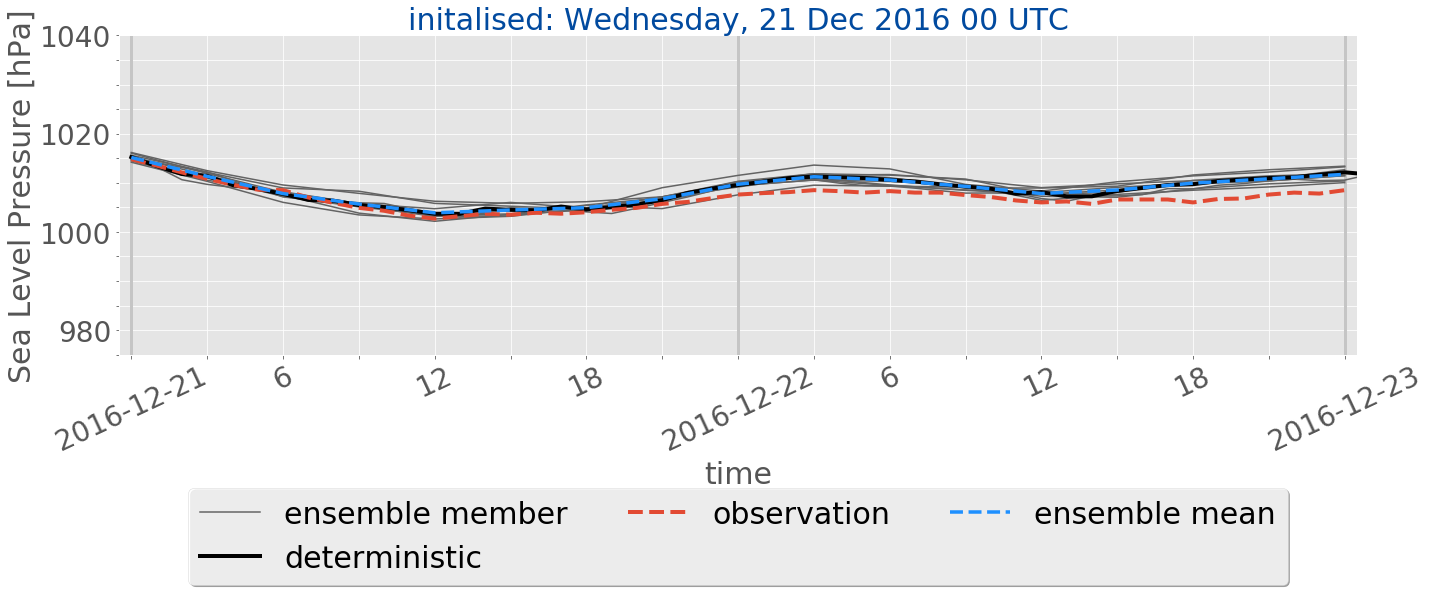
\includegraphics[trim={0.cm 1.5cm 0cm 0cm},clip,
		width=\textwidth]{./fig_sfc_pressure/20161221_00}
		\caption{}\label{fig:res:sfc_pres21}
	\end{subfigure}
	% sfc temp
	\begin{subfigure}[b]{0.9\textwidth}
		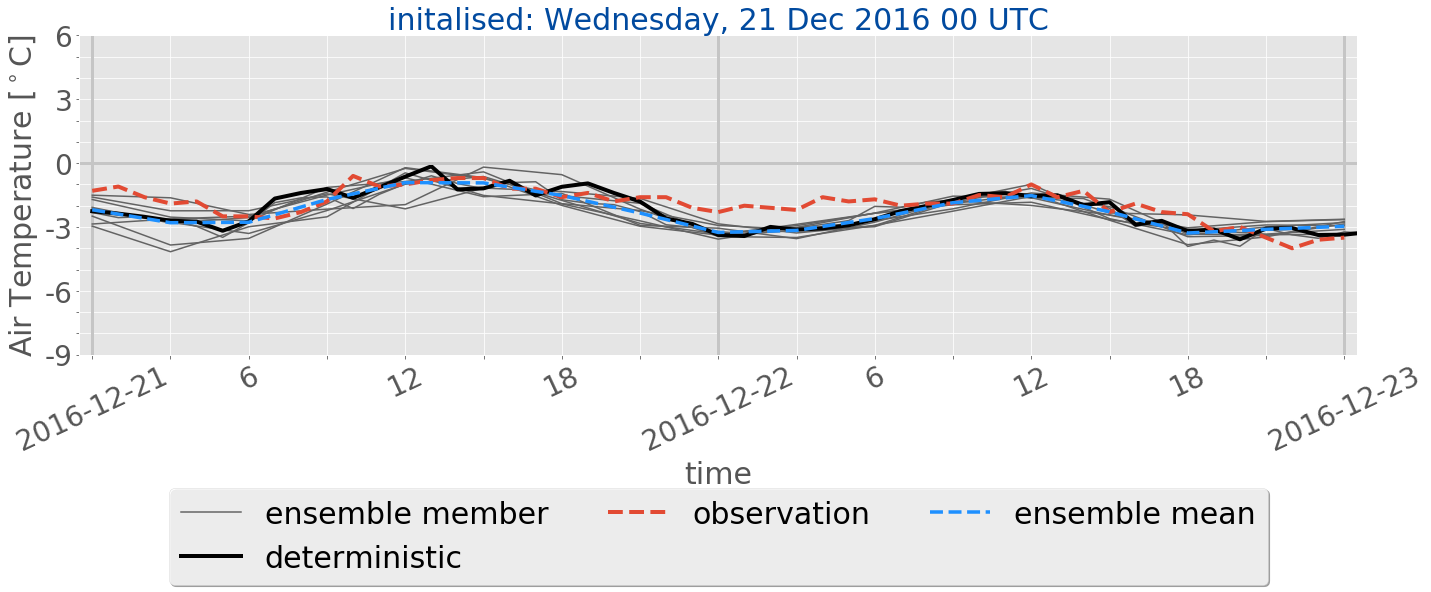
\includegraphics[trim={0.cm 1.5cm 0cm 0cm},clip,
		width=\textwidth]{./fig_sfc_temp/20161221_00}
		\caption{}\label{fig:res:sfc_temp21}
	\end{subfigure}
	%
	% sfc wd
	\begin{subfigure}[b]{0.9\textwidth}
		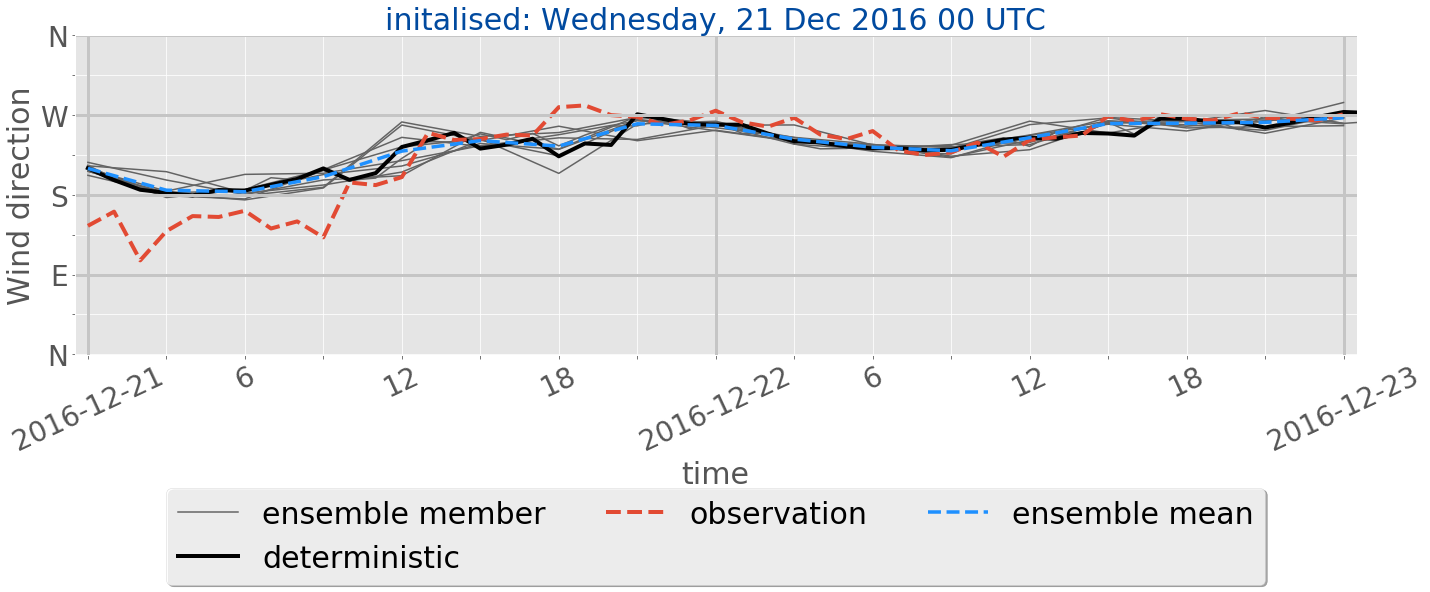
\includegraphics[trim={0.cm 1.5cm 0cm 0cm},clip,
		width=\textwidth]{./fig_sfc_wd/20161221_00}
		\caption{}\label{fig:res:sfc_wd21}
	\end{subfigure}
	% sfc ws
	\begin{subfigure}[b]{0.9\textwidth}
		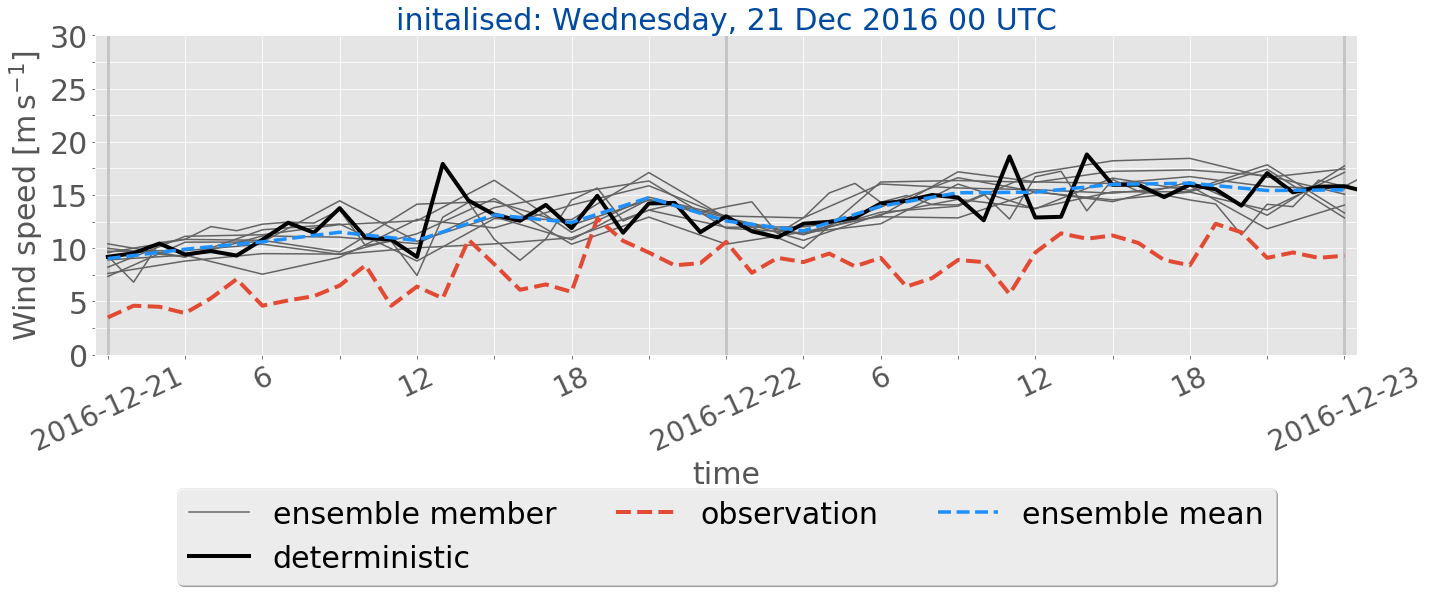
\includegraphics[trim={0.cm 1.5cm 0cm 0cm},clip,
		width=\textwidth]{./fig_sfc_ws/20161221_00}
		\caption{}\label{fig:res:sfc_ws21}
	\end{subfigure}
	% sfc precip
	\begin{subfigure}[b]{0.9\textwidth}
		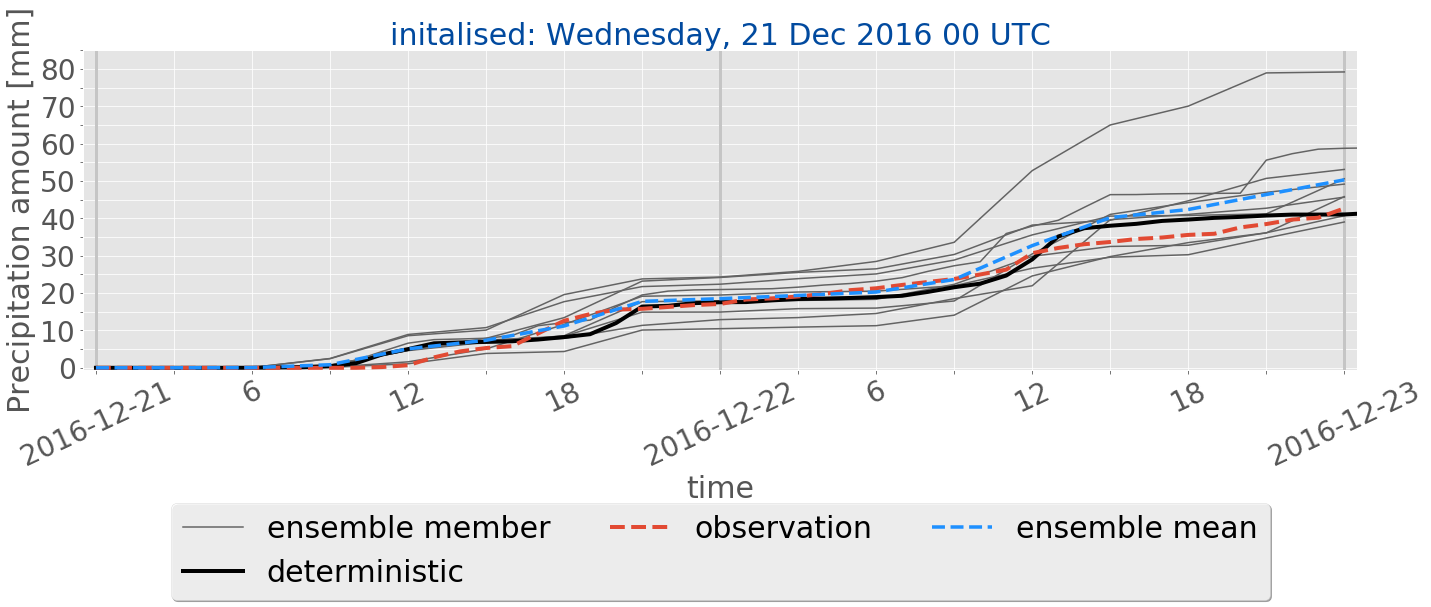
\includegraphics[trim={0.cm 1.5cm 0cm 0cm},clip,
		width=\textwidth]{./fig_sfc_precip/20161221_00}
		\caption{}\label{fig:res:sfc_precip21}
	\end{subfigure}
	% label
	\begin{subfigure}[b]{\textwidth}
		\centering
		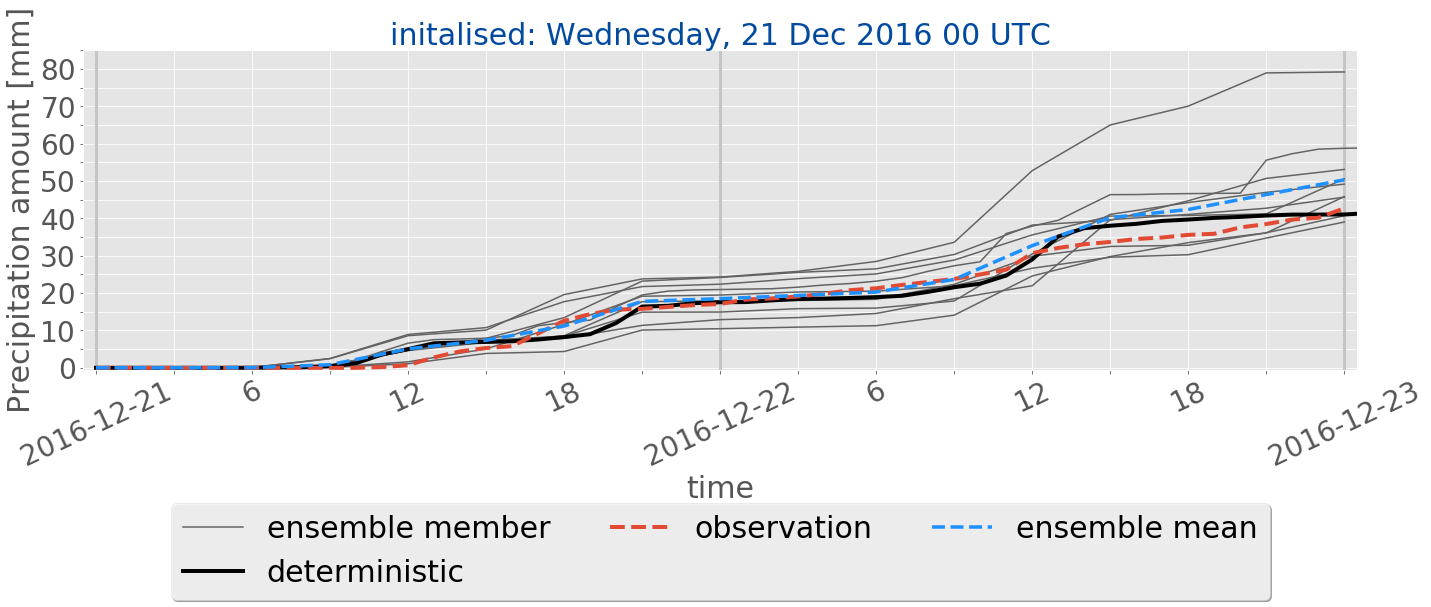
\includegraphics[trim={5.5cm 0cm 5.cm 17.7cm},clip,
		width=0.8\textwidth]{./fig_sfc_precip/20161221_00_label}
	\end{subfigure}
	\caption{\SI{48}{\hour} surface observations and MEPS ensemble forecasts initialised on \SI{21}{\dec} at \SI{0}{\UTC}. 
		Line representation according to the label. From top to bottom: sea level pressure, \SI{2}{\metre} air temperature, \SI{10}{\metre} wind direction and speed, and precipitation amount. \textit{Continued on next page.}}\label{fig:obs_meps:21}
	%
\end{figure}
%%%%%%%%%%%%%%%%%%%%%%%%%%%%%%%%%%%%%%%%%%%%%%%%%%%%%%%%%%%%
%  \begin{figure}[H]%\ContinuedFloat
%  	\centering
%  	% sfc pressure
%  	\begin{subfigure}[b]{0.9\textwidth}
%  		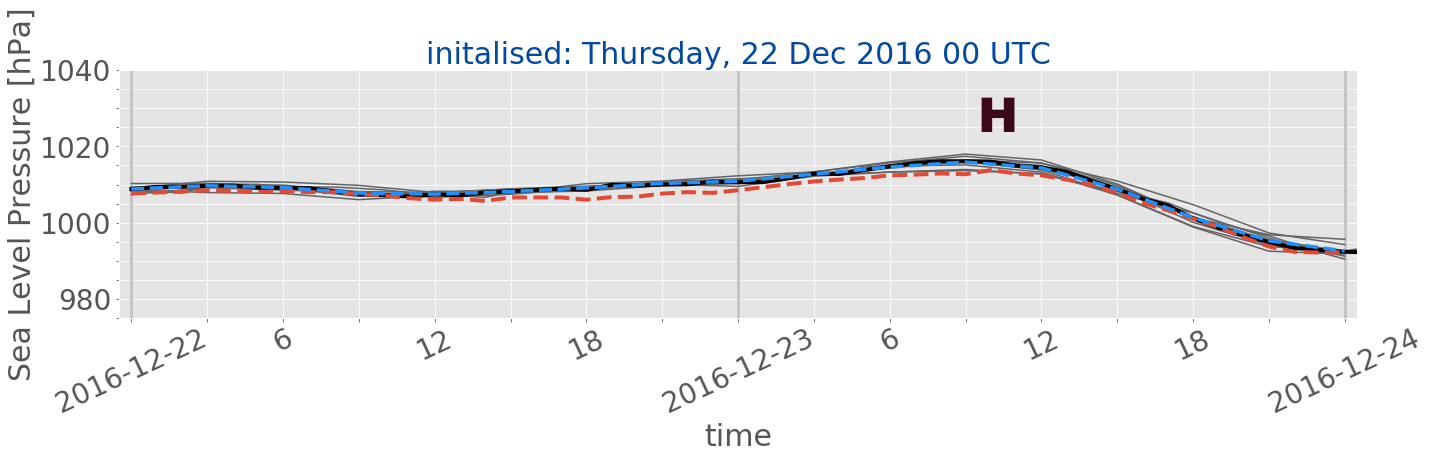
\includegraphics[trim={0.cm 1.5cm 0cm 0cm},clip,
%  		width=\textwidth]{./fig_sfc_pressure/20161222_00}
%  		\caption{}\label{fig:res:sfc_pres22}
%  	\end{subfigure}
%  	% sfc temp
%  	\begin{subfigure}[b]{0.9\textwidth}
%  		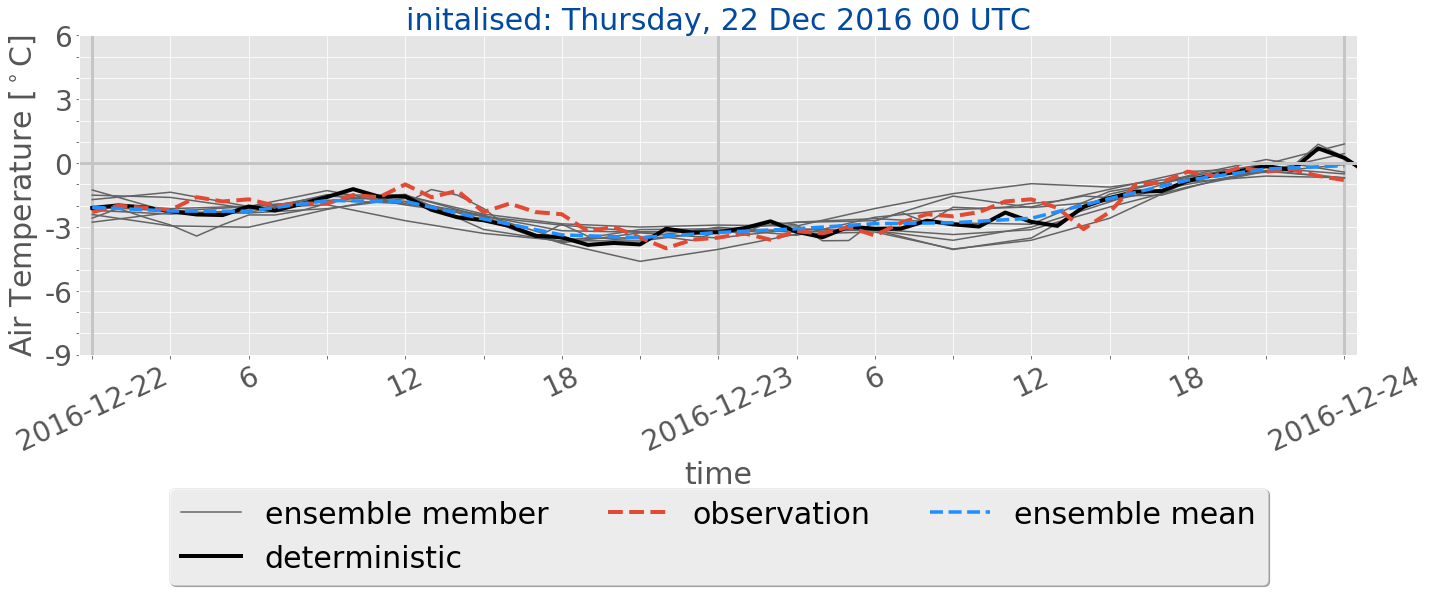
\includegraphics[trim={0.cm 1.5cm 0cm 0cm},clip,
%  		width=\textwidth]{./fig_sfc_temp/20161222_00}
%  		\caption{}\label{fig:res:sfc_temp22}
%  	\end{subfigure}
%  	%
%  	% sfc wd
%  	\begin{subfigure}[b]{0.9\textwidth}
%  		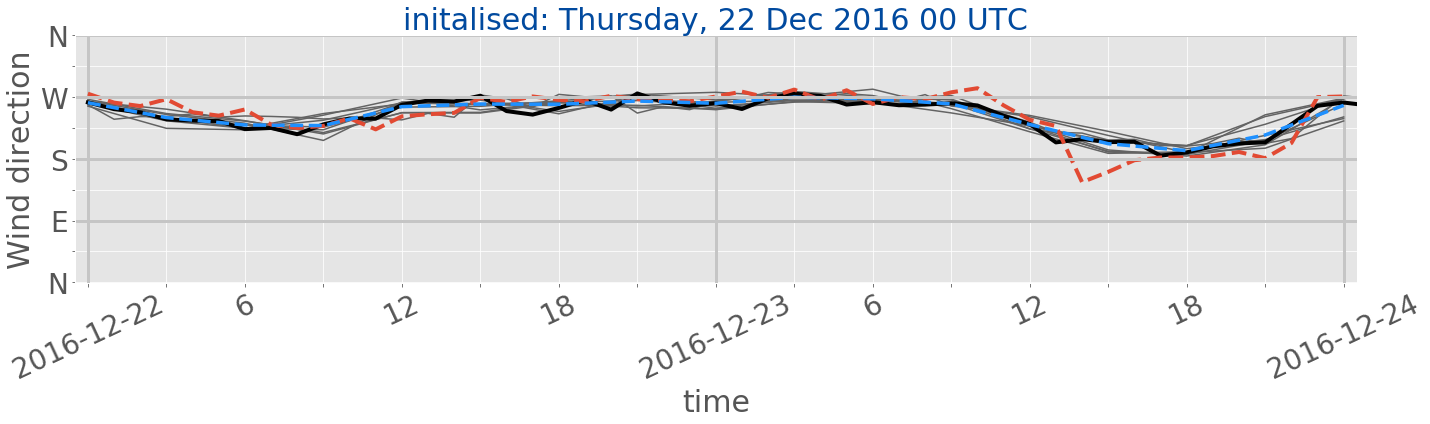
\includegraphics[trim={0.cm 1.5cm 0cm 0cm},clip,
%  		width=\textwidth]{./fig_sfc_wd/20161222_00}
%  		\caption{}\label{fig:res:sfc_wd22}
%  	\end{subfigure}
%  	% sfc ws
%  	\begin{subfigure}[b]{0.9\textwidth}
%  		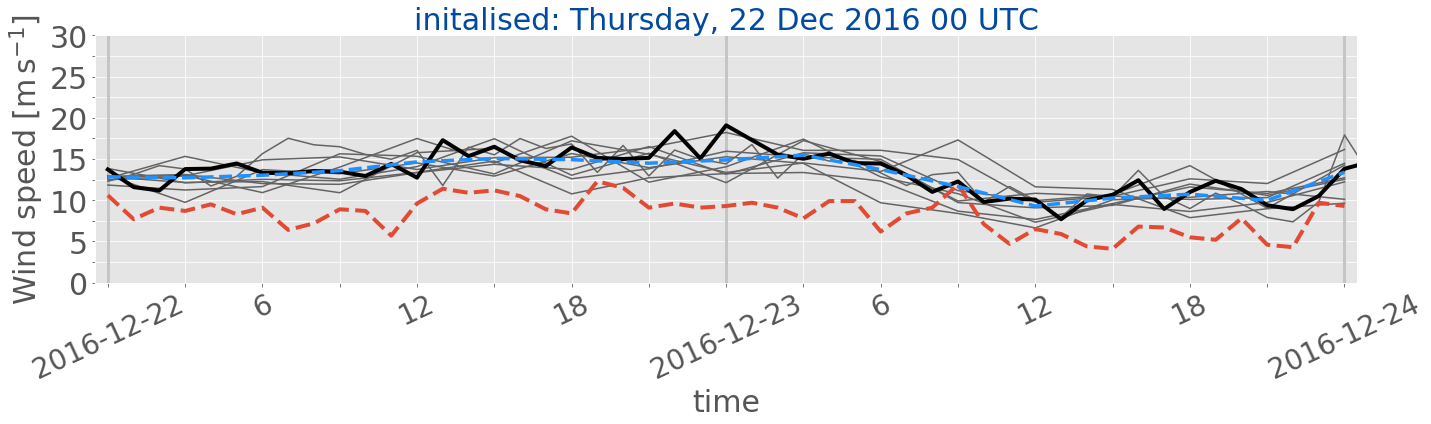
\includegraphics[trim={0.cm 1.5cm 0cm 0cm},clip,
%  		width=\textwidth]{./fig_sfc_ws/20161222_00}
%  		\caption{}\label{fig:res:sfc_ws22}
%  	\end{subfigure}
%  	% sfc precip
%  	\begin{subfigure}[b]{0.9\textwidth}
%  		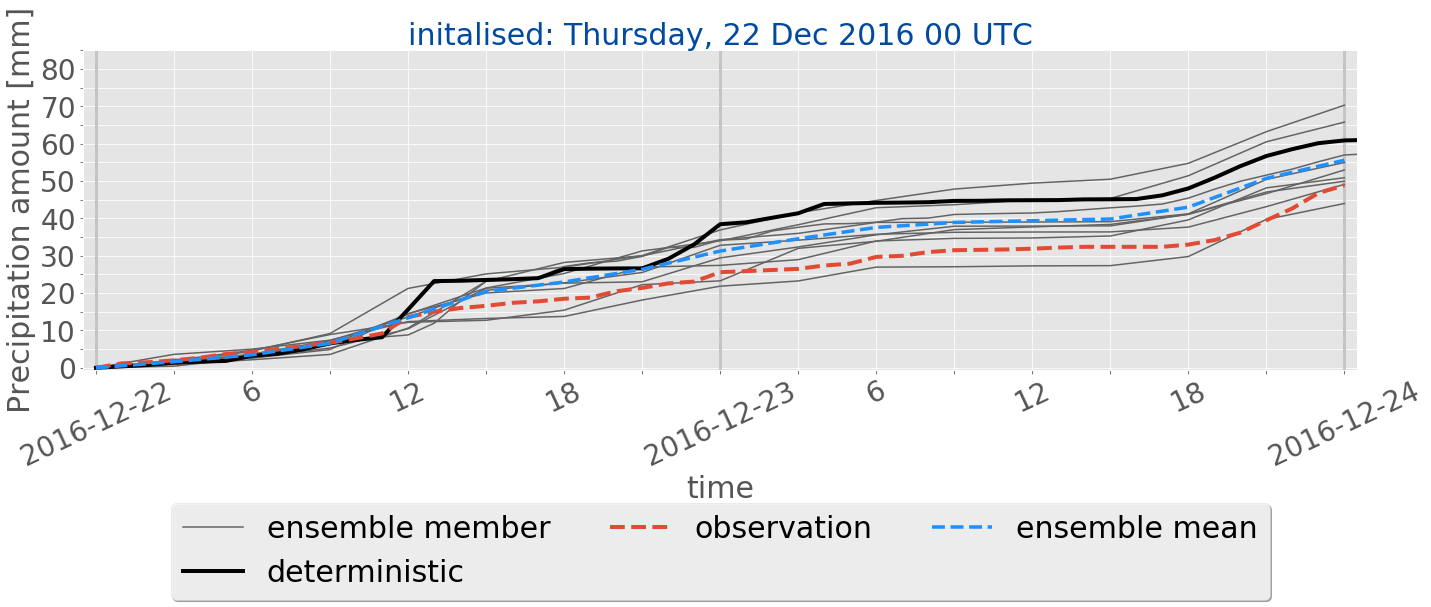
\includegraphics[trim={0.cm 1.5cm 0cm 0cm},clip,
%  		width=\textwidth]{./fig_sfc_precip/20161222_00}
%  		\caption{}\label{fig:res:sfc_precip22}
%  	\end{subfigure}
%  	% label
%  	\begin{subfigure}[b]{\textwidth}
%  		\centering
%  		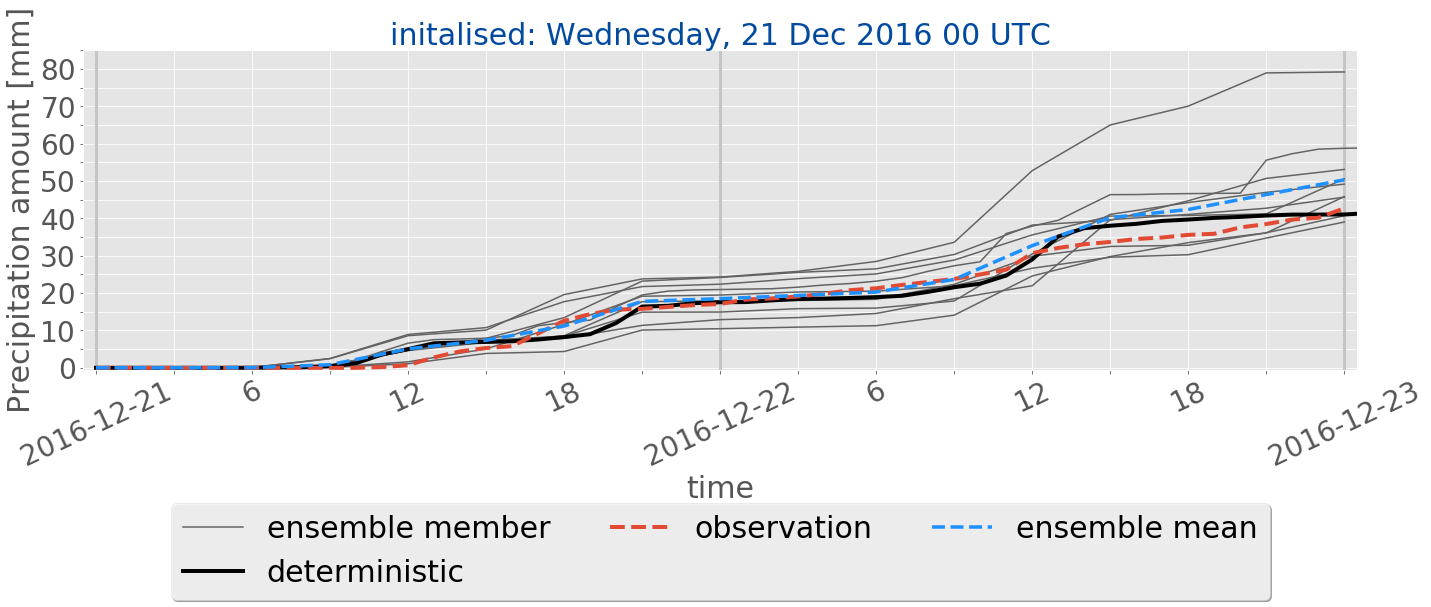
\includegraphics[trim={5.5cm 0cm 5.cm 17.7cm},clip,
%  		width=0.8\textwidth]{./fig_sfc_precip/20161221_00_label}
%  	\end{subfigure}
%  	\caption{\textit{(As \Cref{fig:obs_meps:21}.)} Initialisation on \SI{22}{\dec} at \SI{0}{\UTC}. }\label{fig:obs_meps:22}
%  	%
%  \end{figure}
%%%%%%%%%%%%%%%%%%%%%%%%%%%%%%%%%%%%%%%%%%%%%%%%%%%%%%%%%%%%
\begin{figure}[H]%\ContinuedFloat
	\centering
	% sfc pressure
	\begin{subfigure}[b]{0.9\textwidth}
		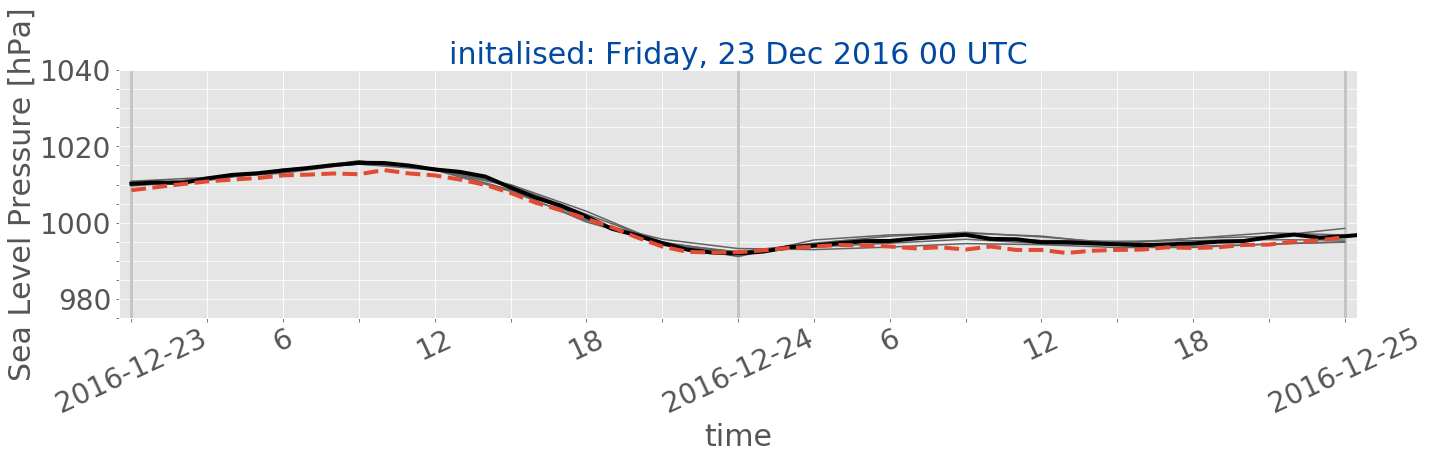
\includegraphics[trim={0.cm 1.5cm 0cm 0cm},clip,
		width=\textwidth]{./fig_sfc_pressure/20161223_00}
		\caption{}\label{fig:res:sfc_pres23}
	\end{subfigure}
	% sfc temp
	\begin{subfigure}[b]{0.9\textwidth}
		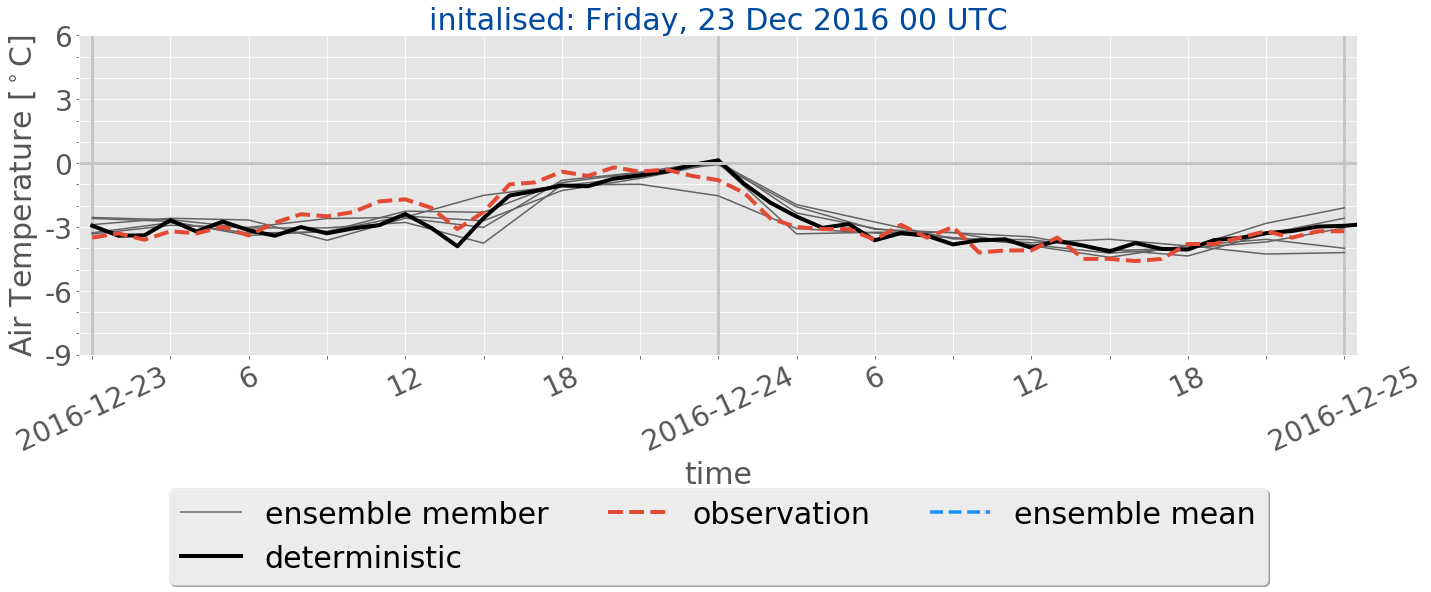
\includegraphics[trim={0.cm 1.5cm 0cm 0cm},clip,
		width=\textwidth]{./fig_sfc_temp/20161223_00}
		\caption{}\label{fig:res:sfc_temp23}
	\end{subfigure}
	%
	% sfc wd
	\begin{subfigure}[b]{0.9\textwidth}
		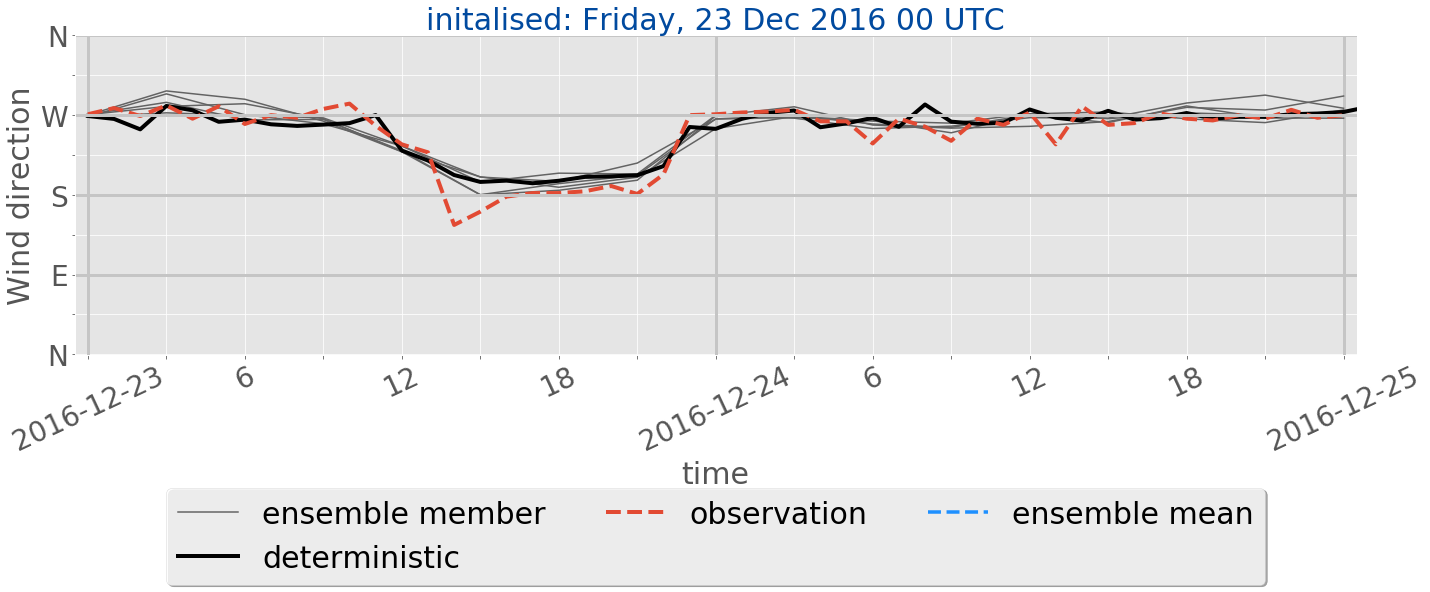
\includegraphics[trim={0.cm 1.5cm 0cm 0cm},clip,
		width=\textwidth]{./fig_sfc_wd/20161223_00}
		\caption{}\label{fig:res:sfc_wd23}
	\end{subfigure}
	% sfc ws
	\begin{subfigure}[b]{0.9\textwidth}
		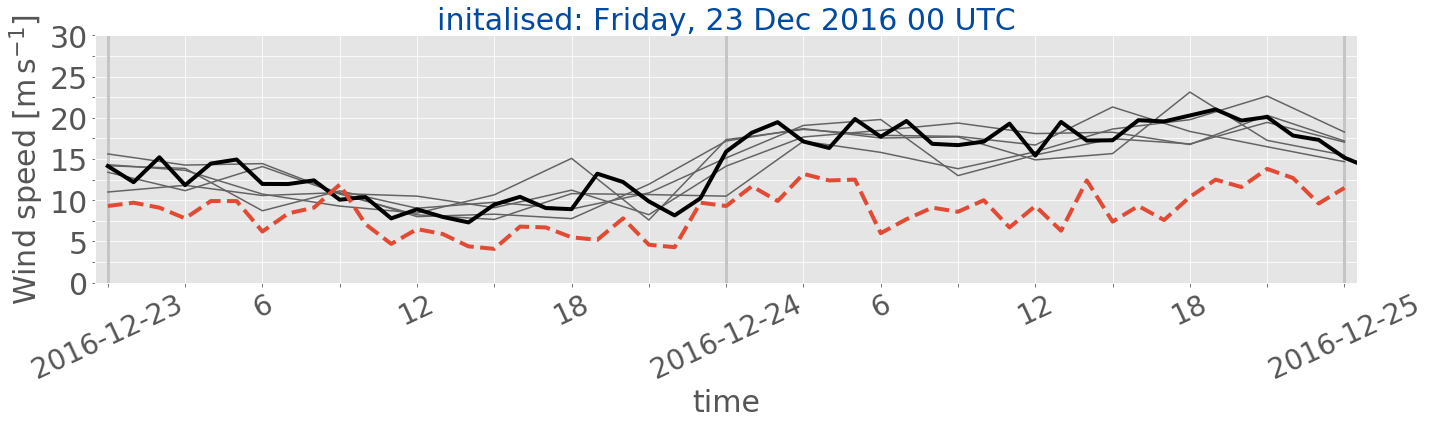
\includegraphics[trim={0.cm 1.5cm 0cm 0cm},clip,
		width=\textwidth]{./fig_sfc_ws/20161223_00}
		\caption{}\label{fig:res:sfc_ws23}
	\end{subfigure}
	% sfc precip
	\begin{subfigure}[b]{0.9\textwidth}
		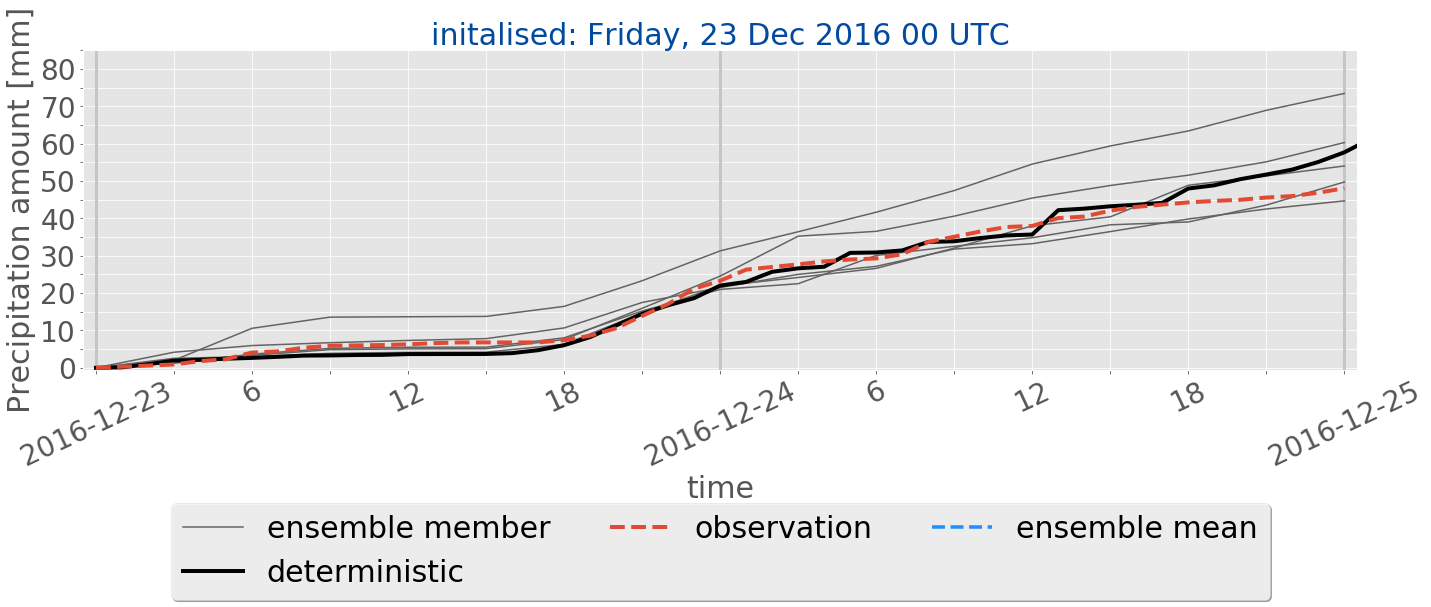
\includegraphics[trim={0.cm 1.5cm 0cm 0cm},clip,
		width=\textwidth]{./fig_sfc_precip/20161223_00}
		\caption{}\label{fig:res:sfc_precip23}
	\end{subfigure}
	% label
	\begin{subfigure}[b]{\textwidth}
		\centering
		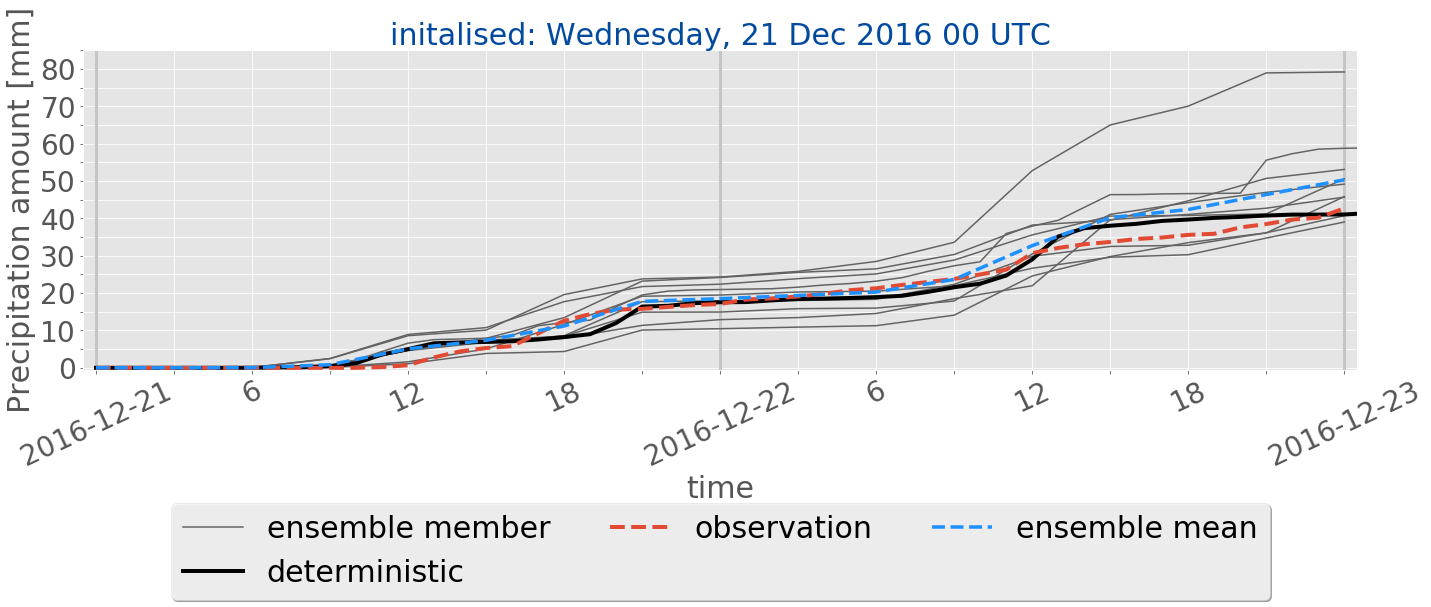
\includegraphics[trim={5.5cm 0cm 5.cm 17.7cm},clip,
		width=0.8\textwidth]{./fig_sfc_precip/20161221_00_label}
	\end{subfigure}
	\caption{\textit{(As \Cref{fig:obs_meps:21}.)} Initialisation on \SI{23}{\dec} at \SI{0}{\UTC}. }\label{fig:obs_meps:23}
	%
\end{figure}
%%%%%%%%%%%%%%%%%%%%%%%%%%%%%%%%%%%%%%%%%%%%%%%%%%%%%%%%%%%%
%  \begin{figure}[H]%\ContinuedFloat
%  	\centering
%  	% sfc pressure
%  	\begin{subfigure}[b]{0.9\textwidth}
%  		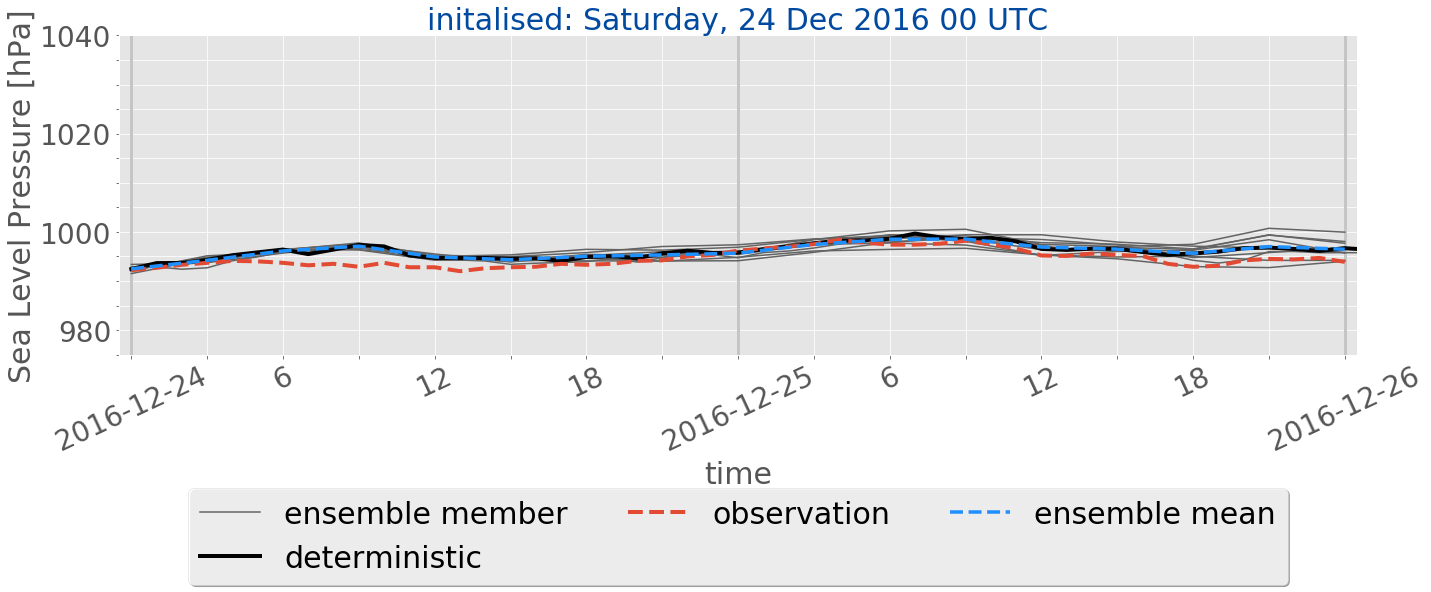
\includegraphics[trim={0.cm 1.5cm 0cm 0cm},clip,
%  		width=\textwidth]{./fig_sfc_pressure/20161224_00}
%  		\caption{}\label{fig:res:sfc_pres24}
%  	\end{subfigure}
%  	% sfc temp
%  	\begin{subfigure}[b]{0.9\textwidth}
%  		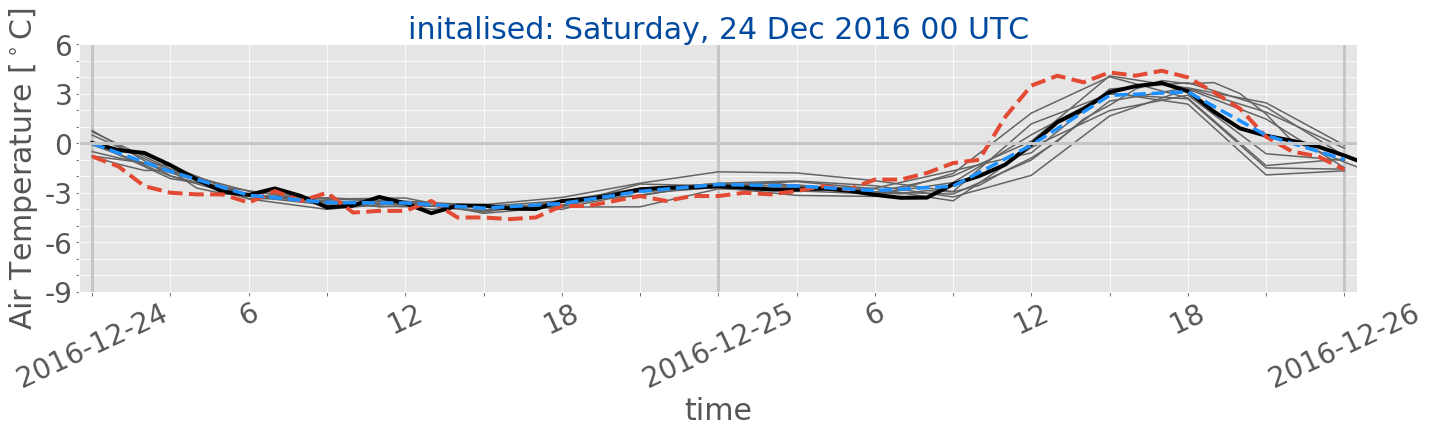
\includegraphics[trim={0.cm 1.5cm 0cm 0cm},clip,
%  		width=\textwidth]{./fig_sfc_temp/20161224_00}
%  		\caption{}\label{fig:res:sfc_temp24}
%  	\end{subfigure}
%  	%
%  	% sfc wd
%  	\begin{subfigure}[b]{0.9\textwidth}
%  		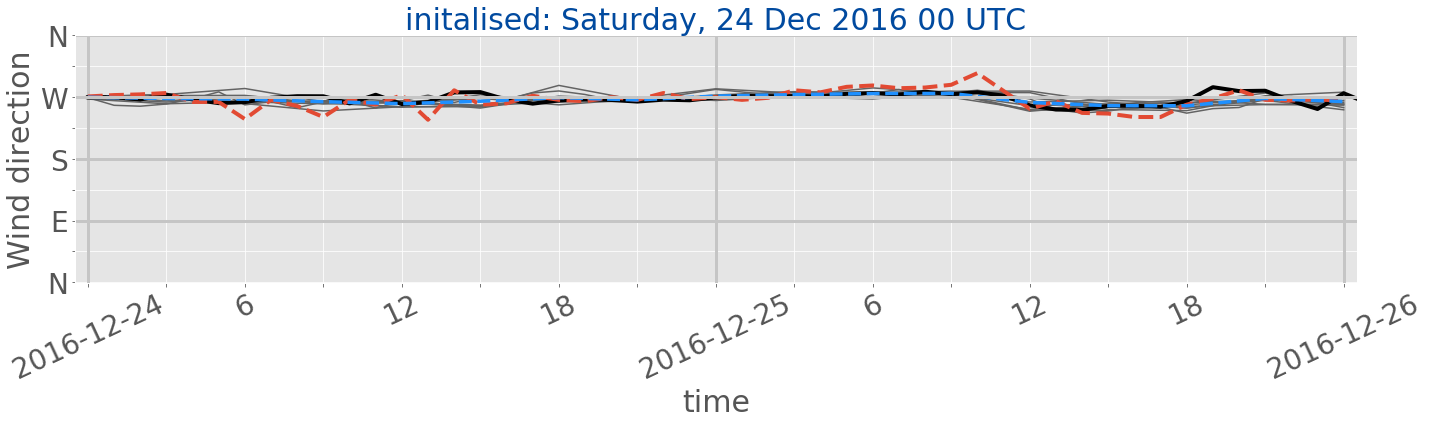
\includegraphics[trim={0.cm 1.5cm 0cm 0cm},clip,
%  		width=\textwidth]{./fig_sfc_wd/20161224_00}
%  		\caption{}\label{fig:res:sfc_wd24}
%  	\end{subfigure}
%  	% sfc ws
%  	\begin{subfigure}[b]{0.9\textwidth}
%  		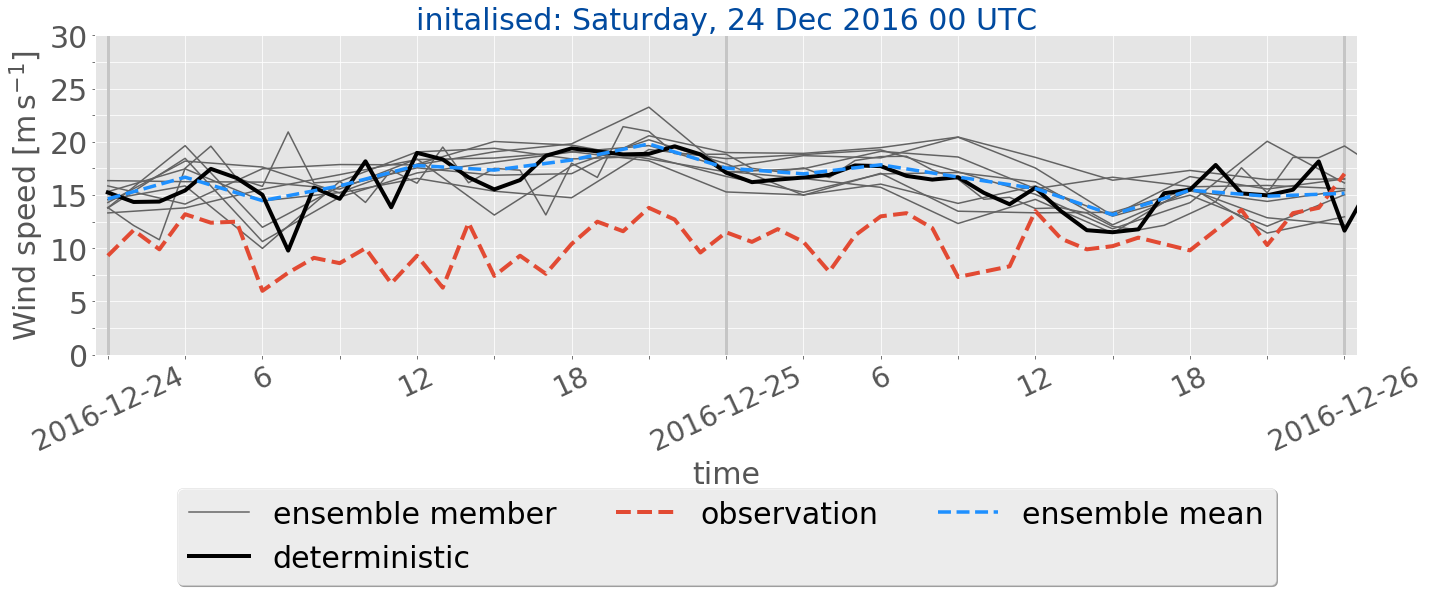
\includegraphics[trim={0.cm 1.5cm 0cm 0cm},clip,
%  		width=\textwidth]{./fig_sfc_ws/20161224_00}
%  		\caption{}\label{fig:res:sfc_ws24}
%  	\end{subfigure}
%  	% sfc precip
%  	\begin{subfigure}[b]{0.9\textwidth}
%  		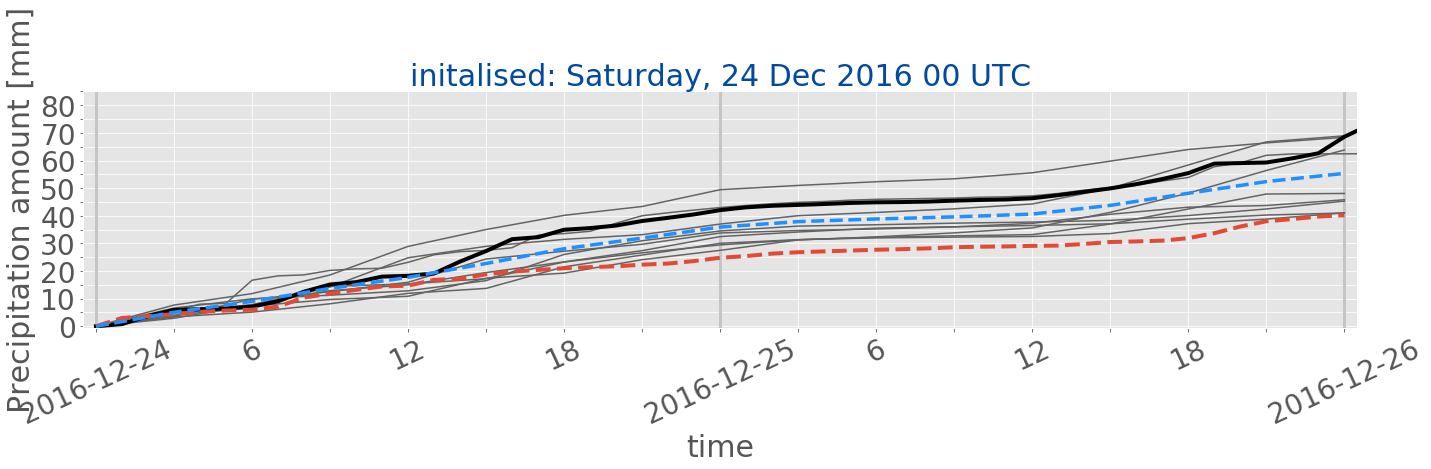
\includegraphics[trim={0.cm 1.5cm 0cm 0cm},clip,
%  		width=\textwidth]{./fig_sfc_precip/20161224_00}
%  		\caption{}\label{fig:res:sfc_precip24}
%  	\end{subfigure}
%  	% label
%  	\begin{subfigure}[b]{\textwidth}
%  		\centering
%  		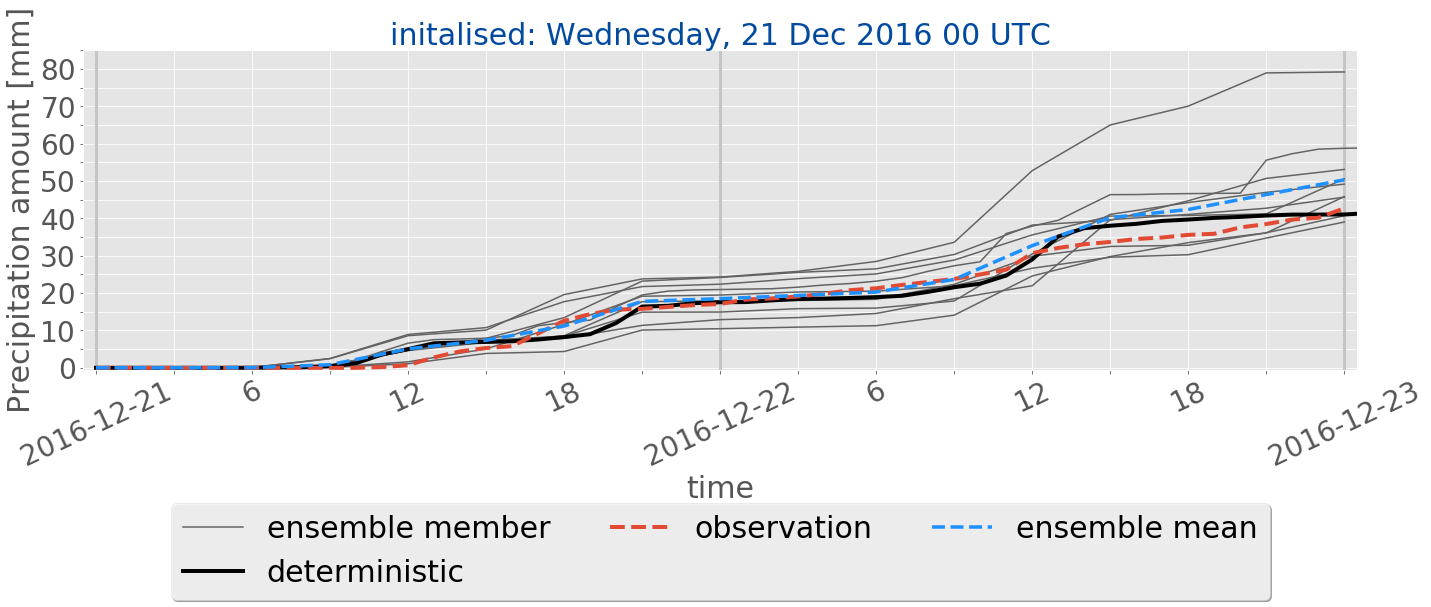
\includegraphics[trim={5.5cm 0cm 5.cm 17.7cm},clip,
%  		width=0.8\textwidth]{./fig_sfc_precip/20161221_00_label}
%  	\end{subfigure}
%  	\caption{\textit{(As \Cref{fig:obs_meps:21}.)} Initialisation on \SI{24}{\dec} at \SI{0}{\UTC}. }\label{fig:obs_meps:24}
%  	%
%  \end{figure}
%%%%%%%%%%%%%%%%%%%%%%%%%%%%%%%%%%%%%%%%%%%%%%%%%%%%%%%%%%%%
\begin{figure}[H]%\ContinuedFloat
	\centering
	% sfc pressure
	%
	\begin{subfigure}[b]{0.9\textwidth}
		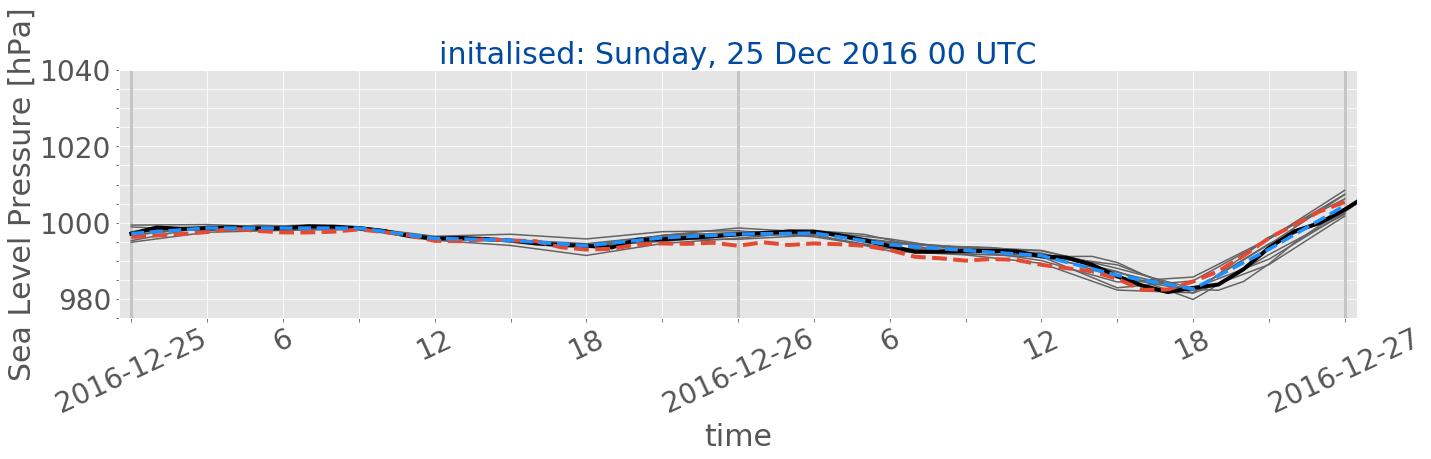
\includegraphics[trim={0.cm 1.5cm 0cm 0cm},clip,
		width=\textwidth]{./fig_sfc_pressure/20161225_00}
		\caption{}\label{fig:res:sfc_pres25}
	\end{subfigure}
	% sfc temp
	%
	\begin{subfigure}[b]{0.9\textwidth}
		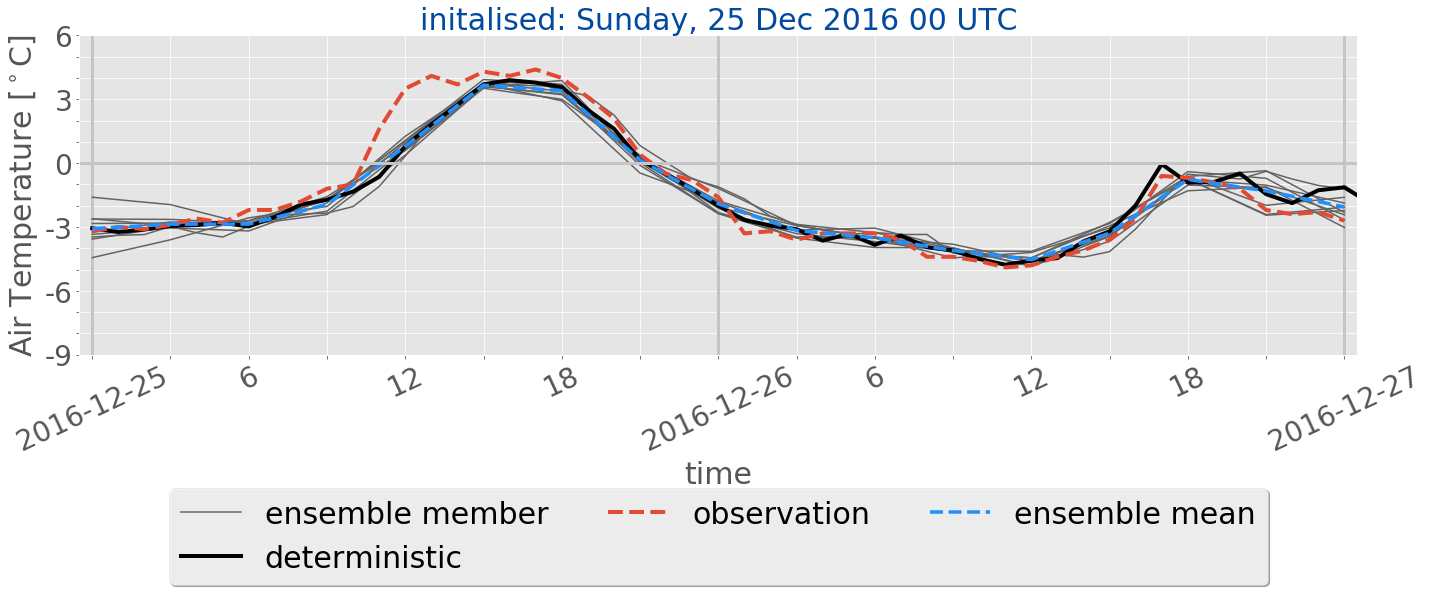
\includegraphics[trim={0.cm 1.5cm 0cm 0cm},clip,
		width=\textwidth]{./fig_sfc_temp/20161225_00}
		\caption{}\label{fig:res:sfc_temp25}
	\end{subfigure}
	% sfc wd
	%
	\begin{subfigure}[b]{0.9\textwidth}
		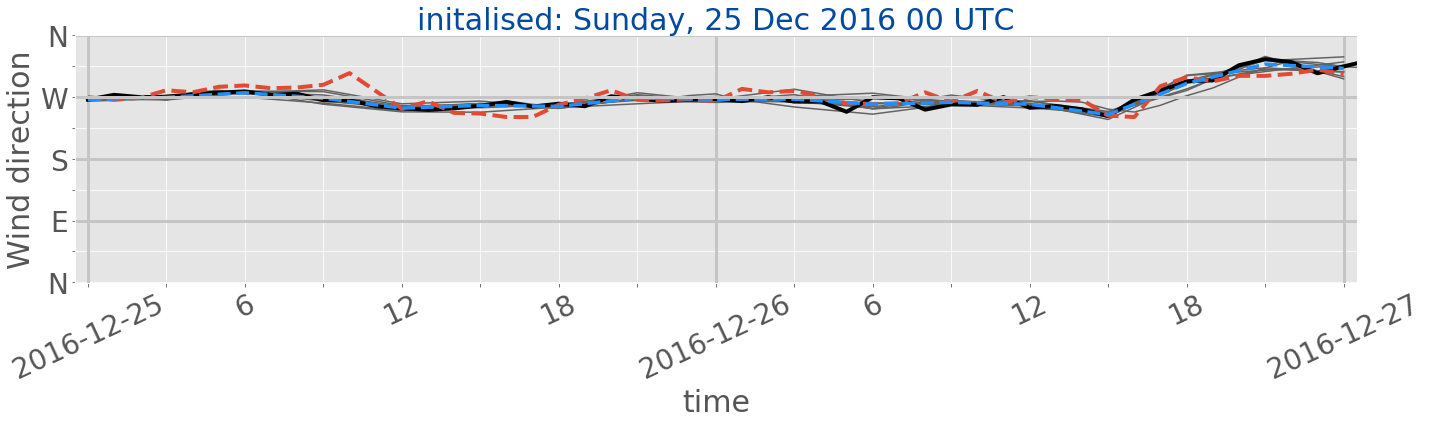
\includegraphics[trim={0.cm 1.5cm 0cm 0cm},clip,
		width=\textwidth]{./fig_sfc_wd/20161225_00}
		\caption{}\label{fig:res:sfc_wd25}
	\end{subfigure}
	% sfc ws
	%
	\begin{subfigure}[b]{0.9\textwidth}
		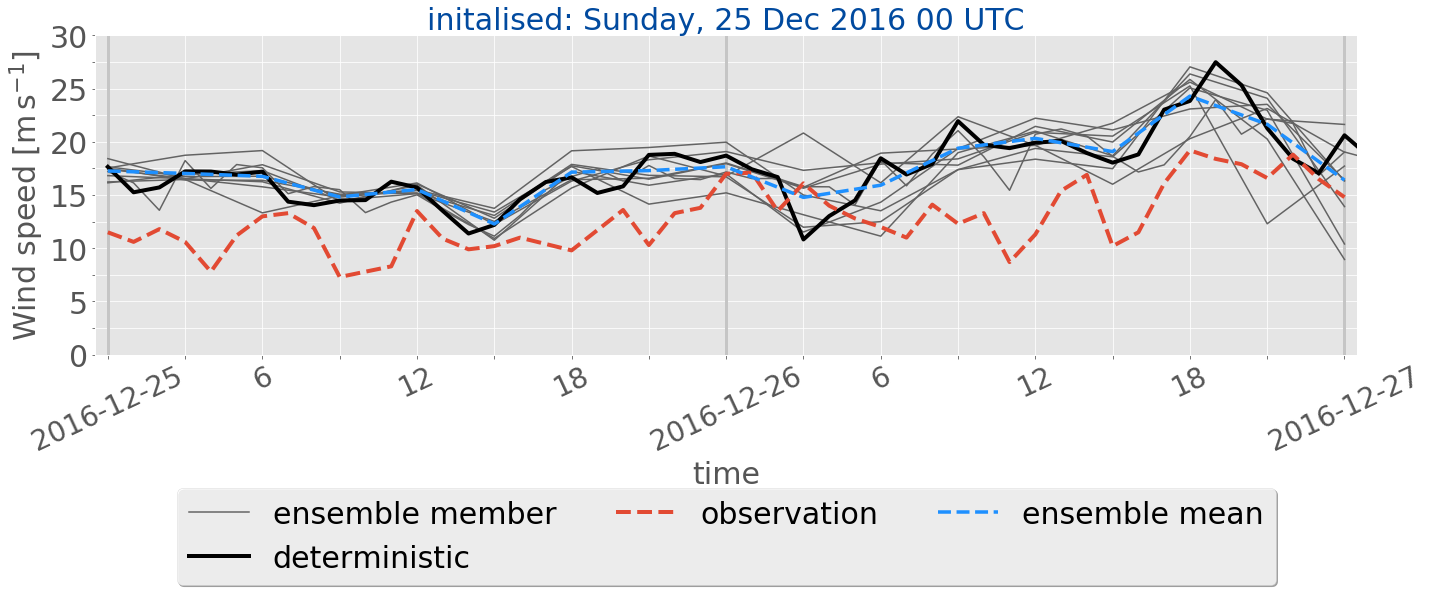
\includegraphics[trim={0.cm 1.5cm 0cm 0cm},clip,
		width=\textwidth]{./fig_sfc_ws/20161225_00}
		\caption{}\label{fig:res:sfc_ws25}
	\end{subfigure}
	% sfc precip
	%
	\begin{subfigure}[b]{0.9\textwidth}
		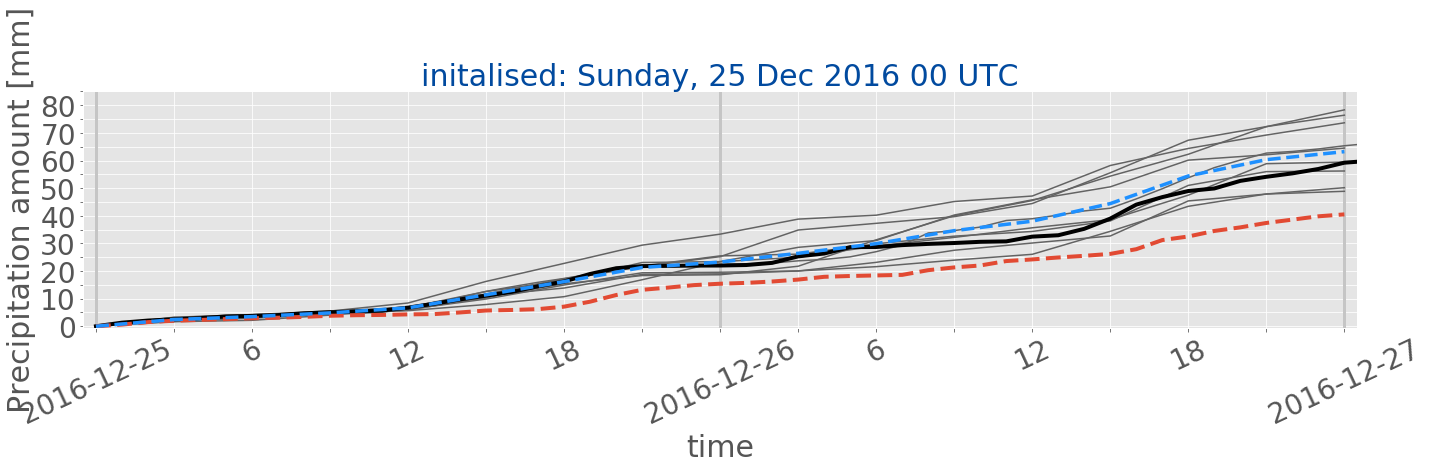
\includegraphics[trim={0.cm 1.5cm 0cm 0cm},clip,
		width=\textwidth]{./fig_sfc_precip/20161225_00}
		\caption{}\label{fig:res:sfc_precip25}
	\end{subfigure}
	% label
	\begin{subfigure}[b]{\textwidth}
		\centering
		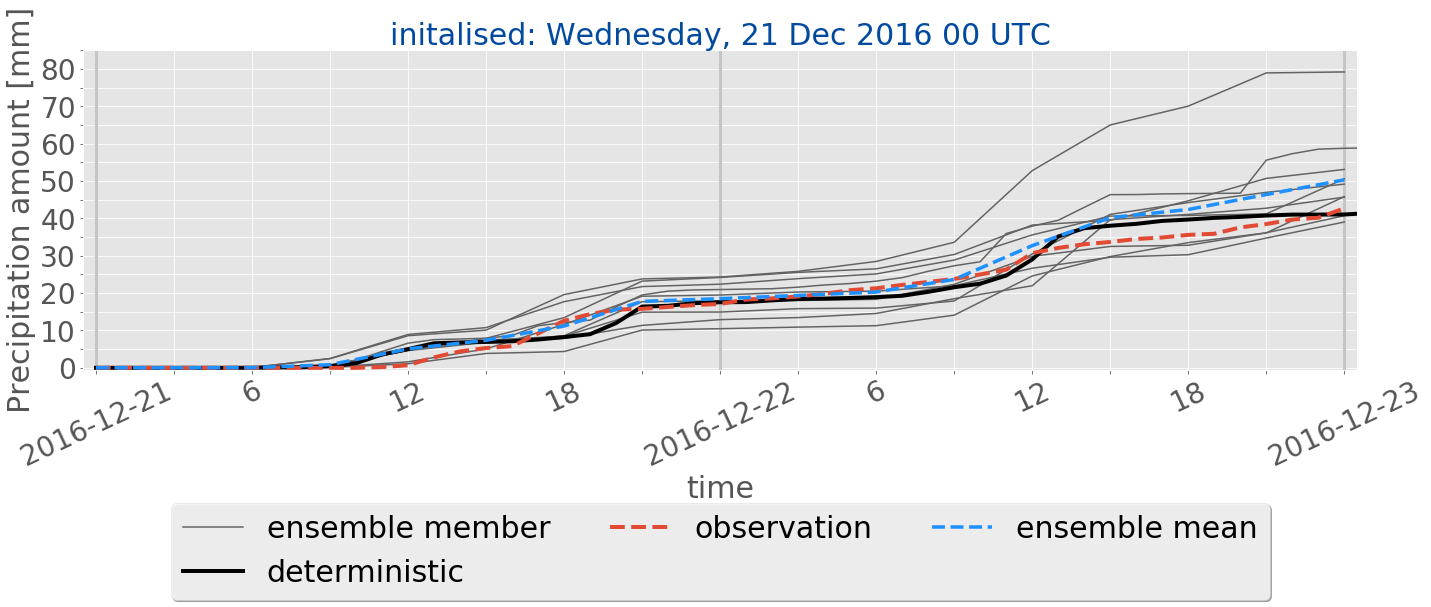
\includegraphics[trim={5.5cm 0cm 5.cm 17.7cm},clip,
		width=0.8\textwidth]{./fig_sfc_precip/20161221_00_label}
	\end{subfigure}
	\caption{\textit{(As \Cref{fig:obs_meps:21}.)} Initialisation on \SI{25}{\dec} at \SI{0}{\UTC}.}\label{fig:obs_meps:25}
	%
\end{figure}
%
\begin{figure}[H]%\ContinuedFloat
	\centering
	% sfc pressure
	\begin{subfigure}[b]{0.9\textwidth}
		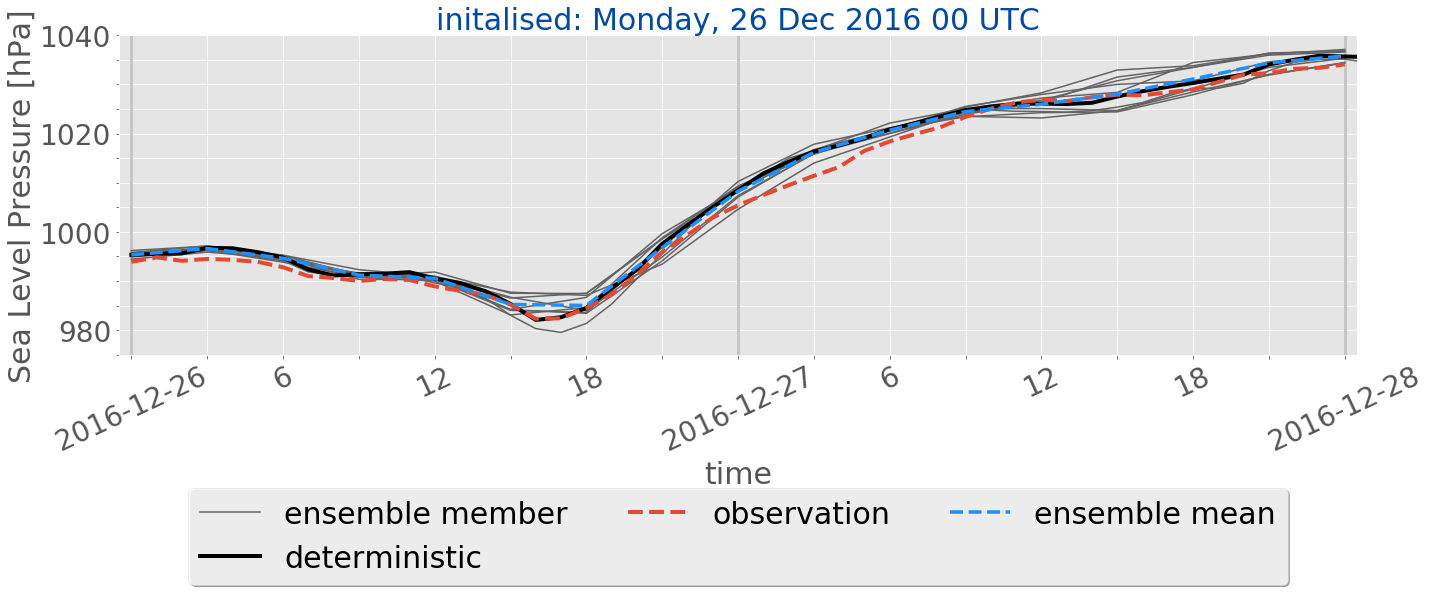
\includegraphics[trim={0.cm 1.5cm 0cm 0cm},clip,
		width=\textwidth]{./fig_sfc_pressure/20161226_00}
		\caption{}\label{fig:res:sfc_pres26}
	\end{subfigure}
	
	% sfc temp
	\begin{subfigure}[b]{0.9\textwidth}
		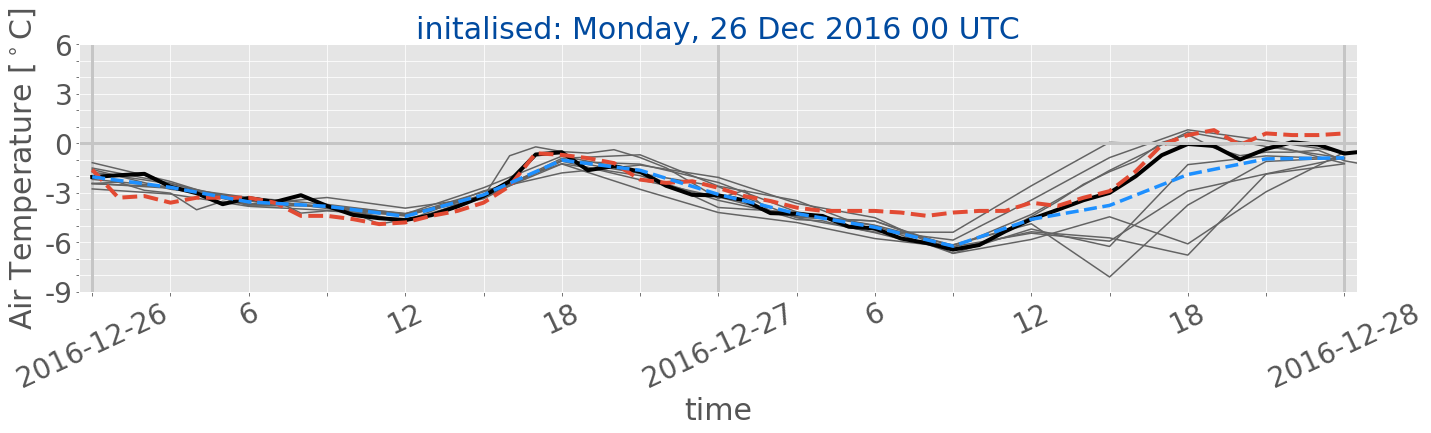
\includegraphics[trim={0.cm 1.5cm 0cm 0cm},clip,
		width=\textwidth]{./fig_sfc_temp/20161226_00}
		\caption{}\label{fig:res:sfc_temp26}
	\end{subfigure}
	%
	% sfc wd
	\begin{subfigure}[b]{0.9\textwidth}
		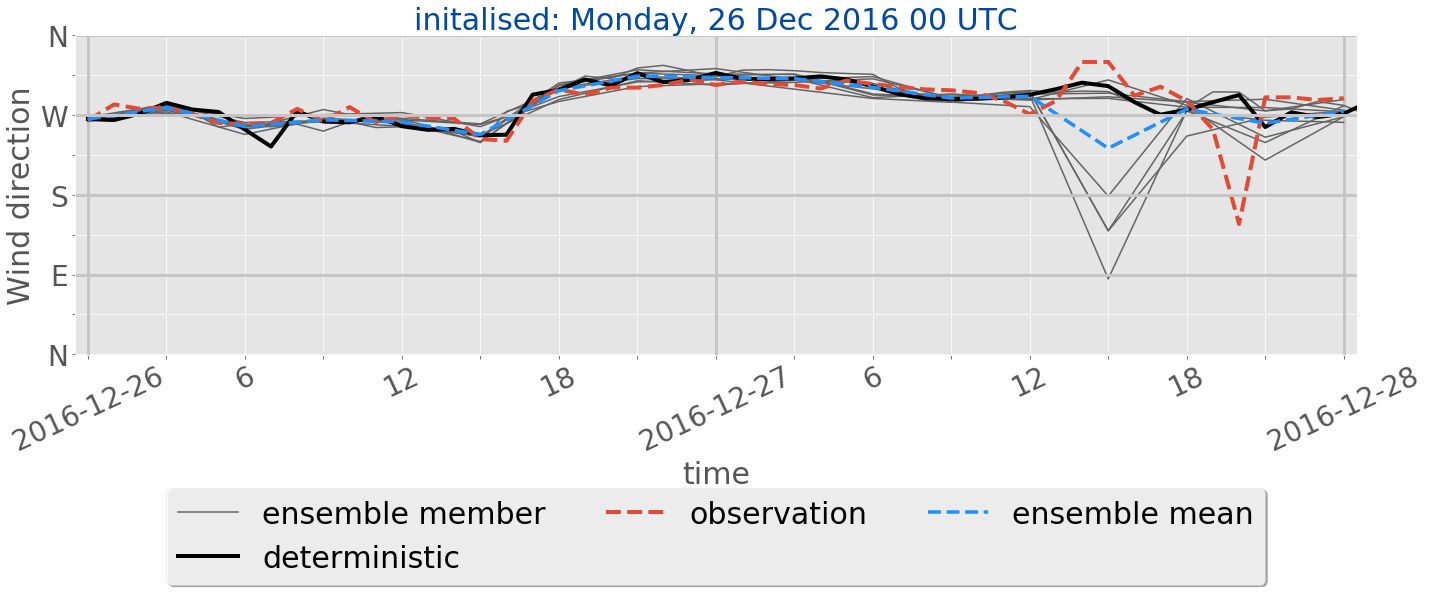
\includegraphics[trim={0.cm 1.5cm 0cm 0cm},clip,
		width=\textwidth]{./fig_sfc_wd/20161226_00}
		\caption{}\label{fig:res:sfc_wd26}
	\end{subfigure}
	%
	% sfc ws
	\begin{subfigure}[b]{0.9\textwidth}
		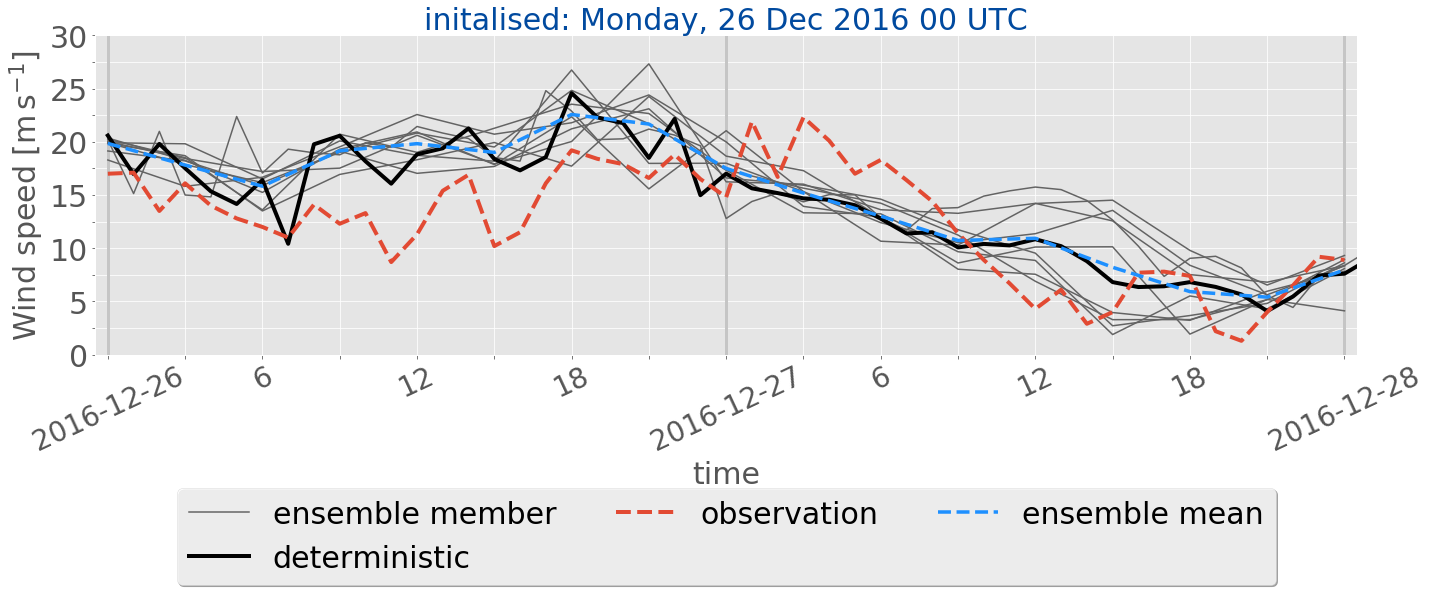
\includegraphics[trim={0.cm 1.5cm 0cm 0cm},clip,
		width=\textwidth]{./fig_sfc_ws/20161226_00}
		\caption{}\label{fig:res:sfc_ws26}
	\end{subfigure}
	%
	% sfc precip
	\begin{subfigure}[b]{0.9\textwidth}
		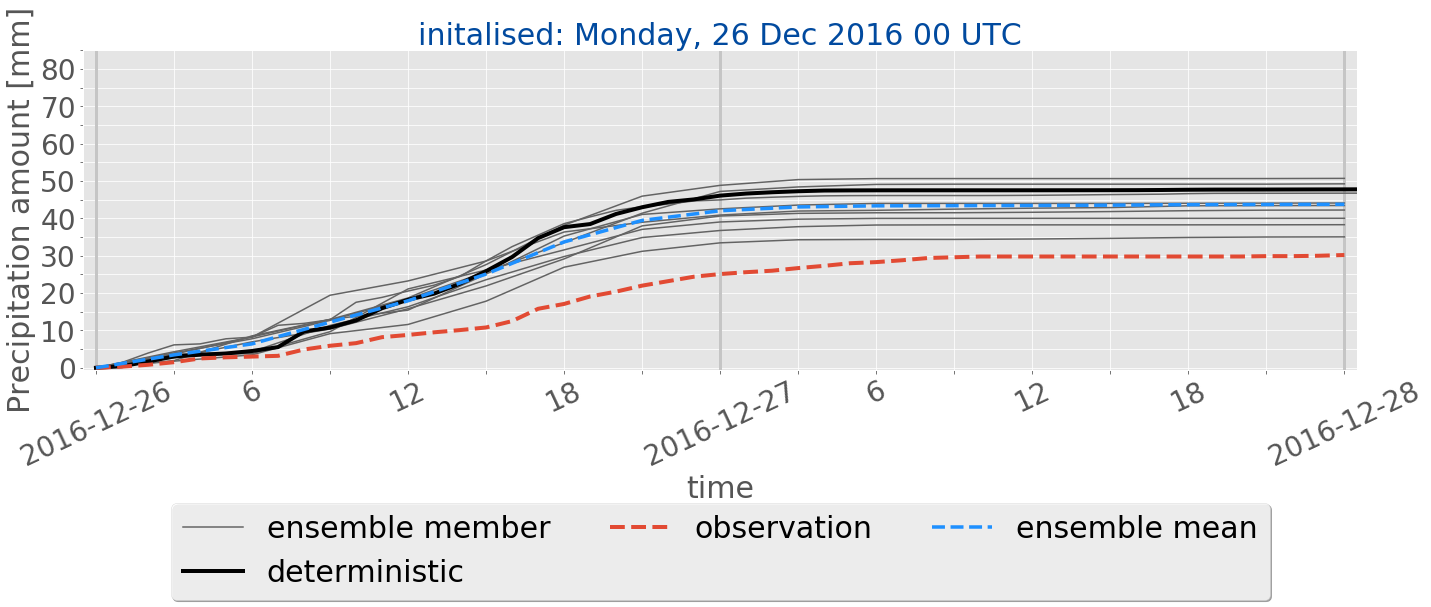
\includegraphics[trim={0.cm 1.5cm 0cm 0cm},clip,
		width=\textwidth]{./fig_sfc_precip/20161226_00}
		\caption{}\label{fig:res:sfc_precip26}
	\end{subfigure}
	% label
	\begin{subfigure}[b]{\textwidth}
		\centering
		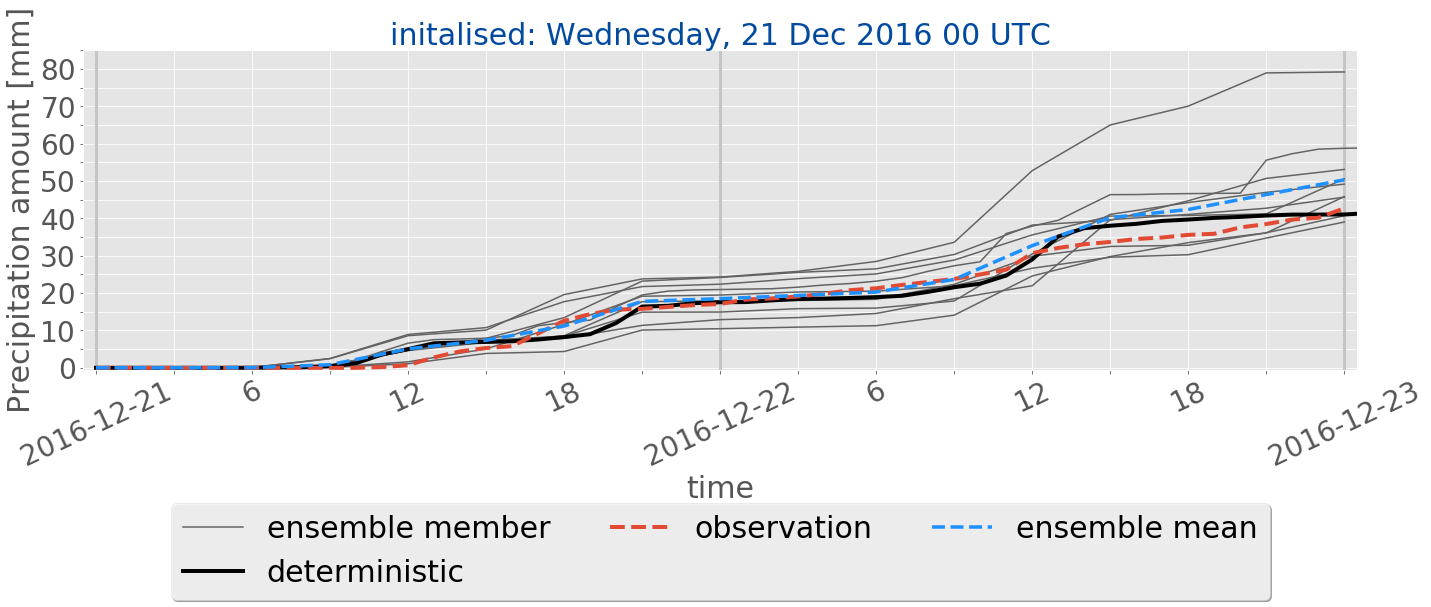
\includegraphics[trim={5.5cm 0cm 5.cm 17.7cm},clip,
		width=0.8\textwidth]{./fig_sfc_precip/20161221_00_label}
	\end{subfigure}
	\caption{\textit{(As \Cref{fig:obs_meps:21}.)} Initialisation on \SI{26}{\dec} at \SI{0}{\UTC}.}\label{fig:obs_meps:26}
\end{figure}
%%%%%%%%%%%%%%%%%%%%%%%%%%%%%%%%%%%%%%%%%%%%%%
%\noindent
%
%%%%%%% image scatter obs ret %%%%%%%%%%%%%%%%
\begin{figure}[t!]
	\centering
	% sfc pressure
	\begin{subfigure}[b]{0.49\textwidth}
		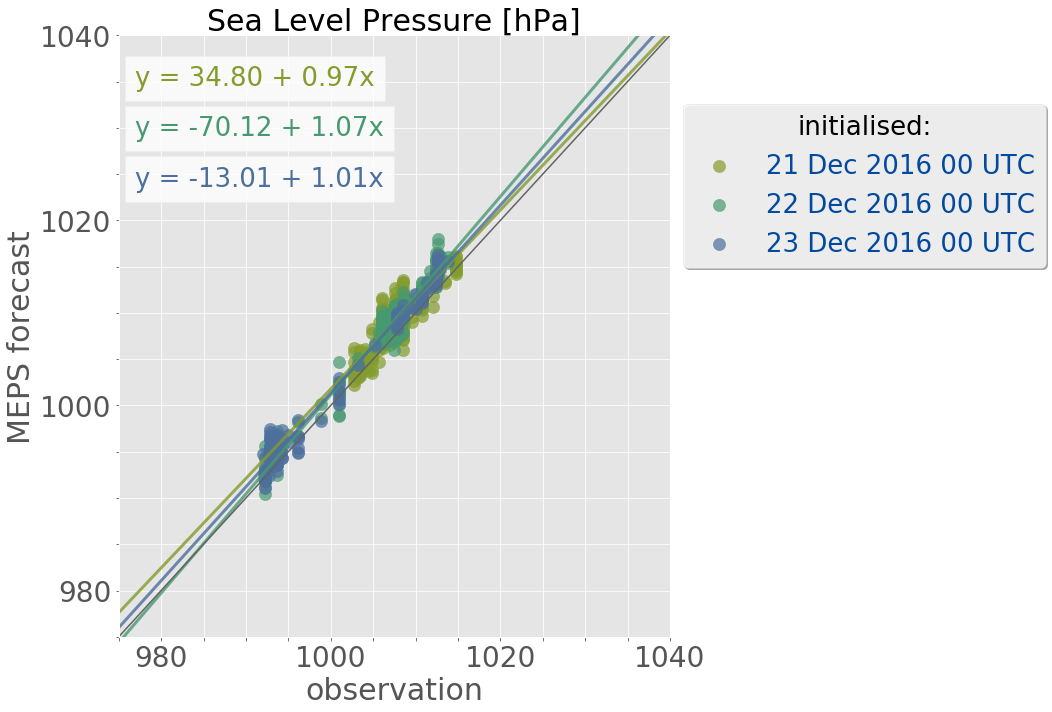
\includegraphics[
		width=\textwidth]{./fig_sfc_pressure/obs_model_20161221_23_00}
		\caption{}\label{fig:scat:pres2123}
	\end{subfigure}
	%
	\begin{subfigure}[b]{0.49\textwidth}
		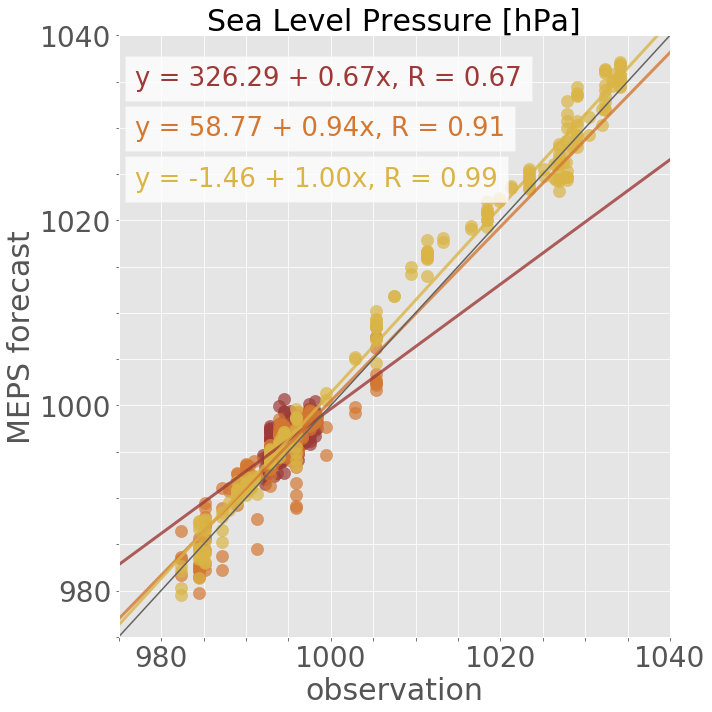
\includegraphics[
		width=\textwidth]{./fig_sfc_pressure/obs_model_20161224_26_00}
		\caption{}\label{fig:scat:pres2426}
	\end{subfigure}
	%
	% label
	\begin{subfigure}[b]{0.49\textwidth}
		\centering
		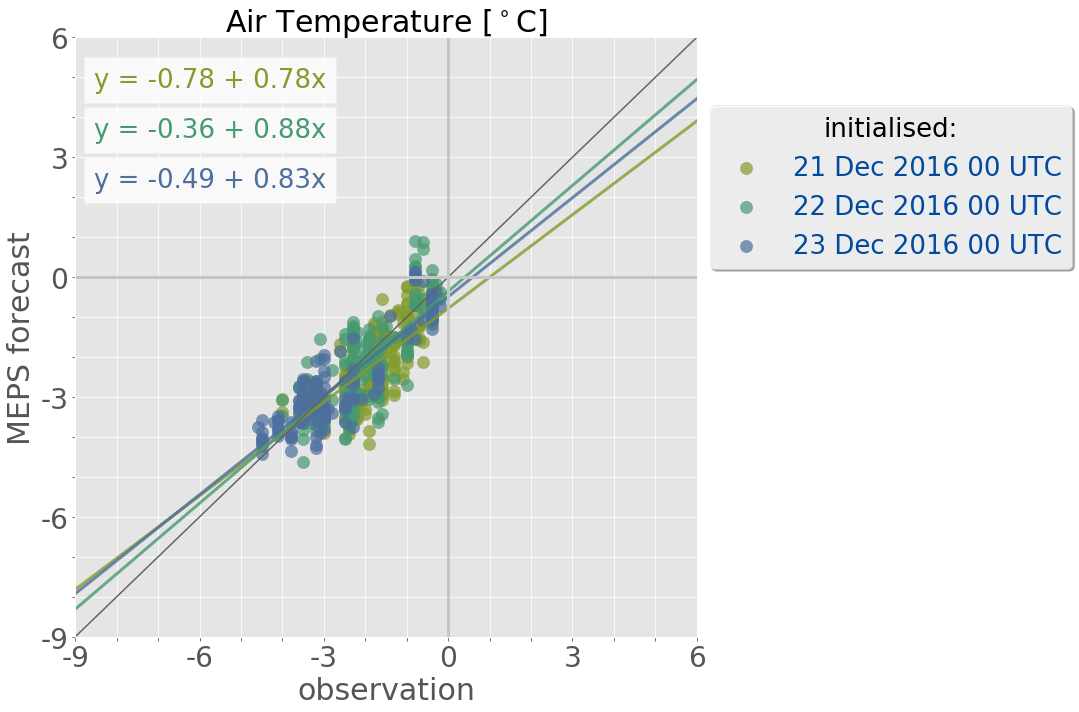
\includegraphics[trim={25.cm 15.5cm 0cm 3.6cm},clip,
		width=0.8\textwidth]{./fig_sfc_temp/obs_model_20161221_23_00_label}
	\end{subfigure}
	\begin{subfigure}[b]{0.49\textwidth}
		\centering
		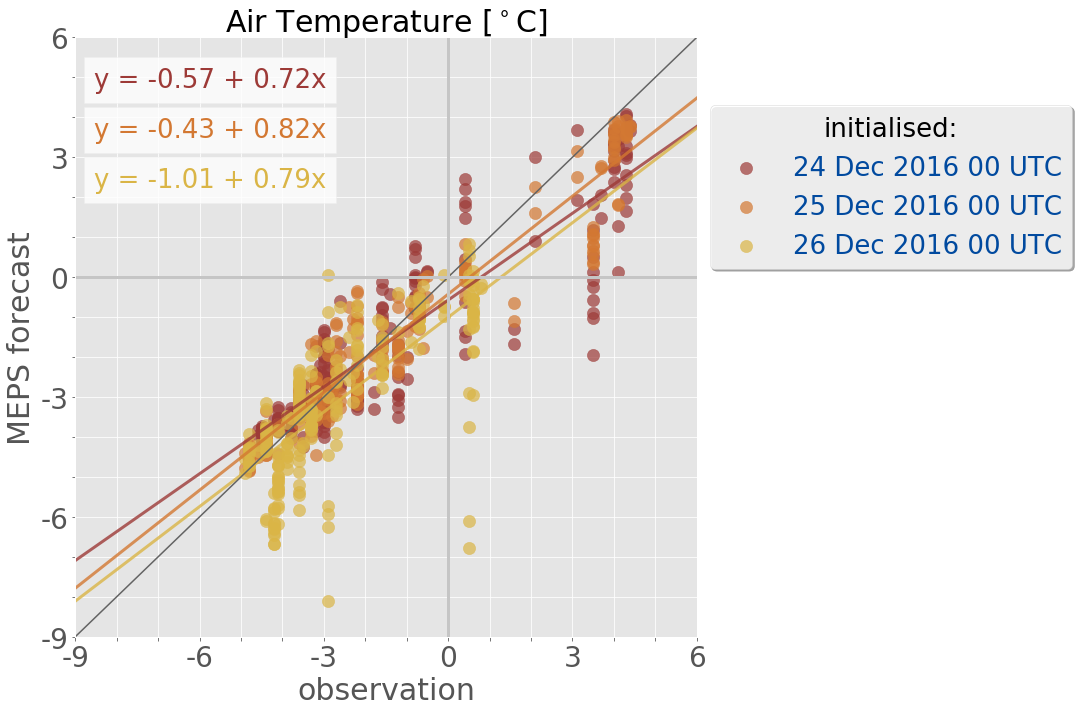
\includegraphics[trim={25.cm 15.5cm 0cm 3.6cm},clip,
		width=0.8\textwidth]{./fig_sfc_temp/obs_model_20161224_26_00_label}
	\end{subfigure}
	\caption{Scatter plots for sea level pressure observations and ensemble forecasts initialised for \num{21} to \SI{23}{\dec} (\protect\subref{fig:scat:pres2123})
    %, \protect\subref{fig:scat:temp2123}, \protect\subref{fig:scat:wd2123}, \protect\subref{fig:scat:ws2123}, \protect\subref{fig:scat:precip2123}) 
    and  for \num{24} ton \SI{26}{\dec} (\protect\subref{fig:scat:pres2426})
    %, \protect\subref{fig:scat:temp2426}, \protect\subref{fig:scat:wd2426}, \protect\subref{fig:scat:ws2426}, \protect\subref{fig:scat:precip2426}). 
    The \SI{48}{\hour} scatter values indicate each day, showing the \SIlist{1;3}{\hour} ten ensemble member forecasts respectively. The linear regression of all ensemble member for each individual day is presented together with the correlation coefficient $R$. %\textit{Continued on next page.}  
    }\label{fig:scat:SLP}
\end{figure}
\begin{figure}%\ContinuedFloat
	\centering
	%     % sfc temp
	\begin{subfigure}[b]{0.49\textwidth}
		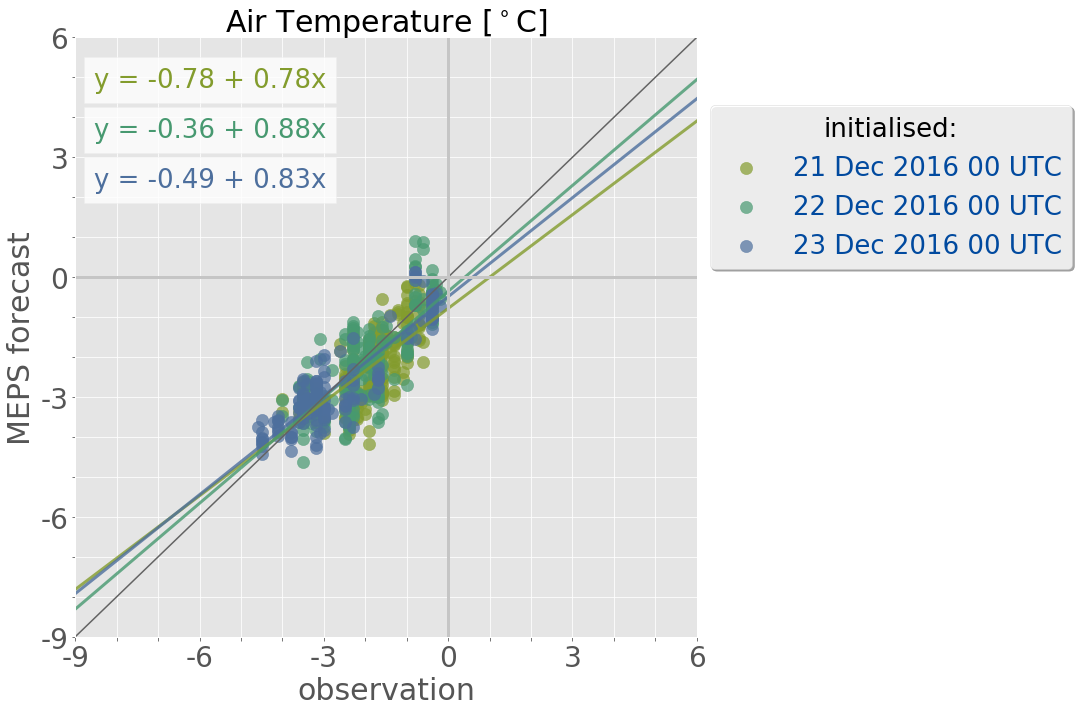
\includegraphics[
		width=\textwidth]{./fig_sfc_temp/obs_model_20161221_23_00}
		\caption{}\label{fig:scat:temp2123}
	\end{subfigure}
	%
	\begin{subfigure}[b]{0.49\textwidth}
		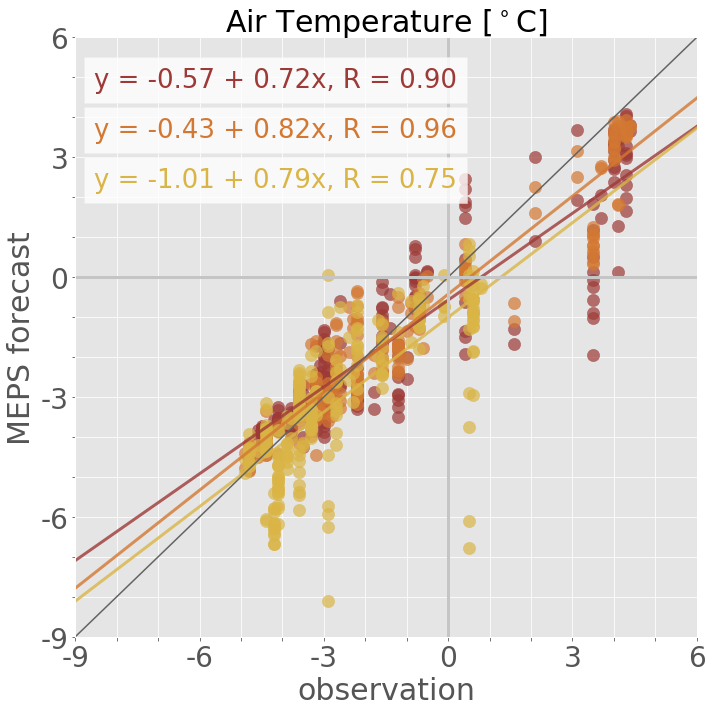
\includegraphics[
		width=\textwidth]{./fig_sfc_temp/obs_model_20161224_26_00}
		\caption{}\label{fig:scat:temp2426}
	\end{subfigure}
	% 
	% sfc wd
	\begin{subfigure}[b]{0.49\textwidth}
		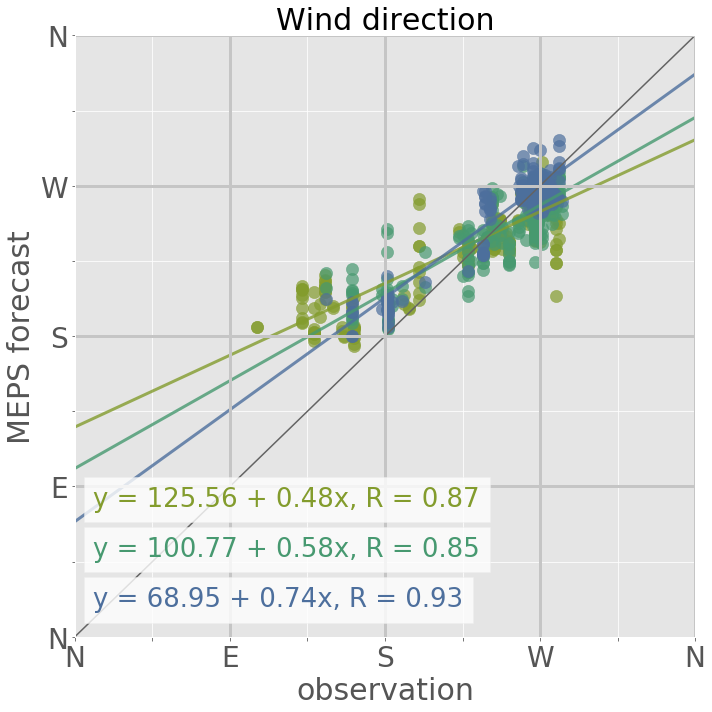
\includegraphics[
		width=\textwidth]{./fig_sfc_wd/obs_model_20161221_23_00}
		\caption{}\label{fig:scat:wd2123}
	\end{subfigure}
	%
	\begin{subfigure}[b]{0.49\textwidth}
		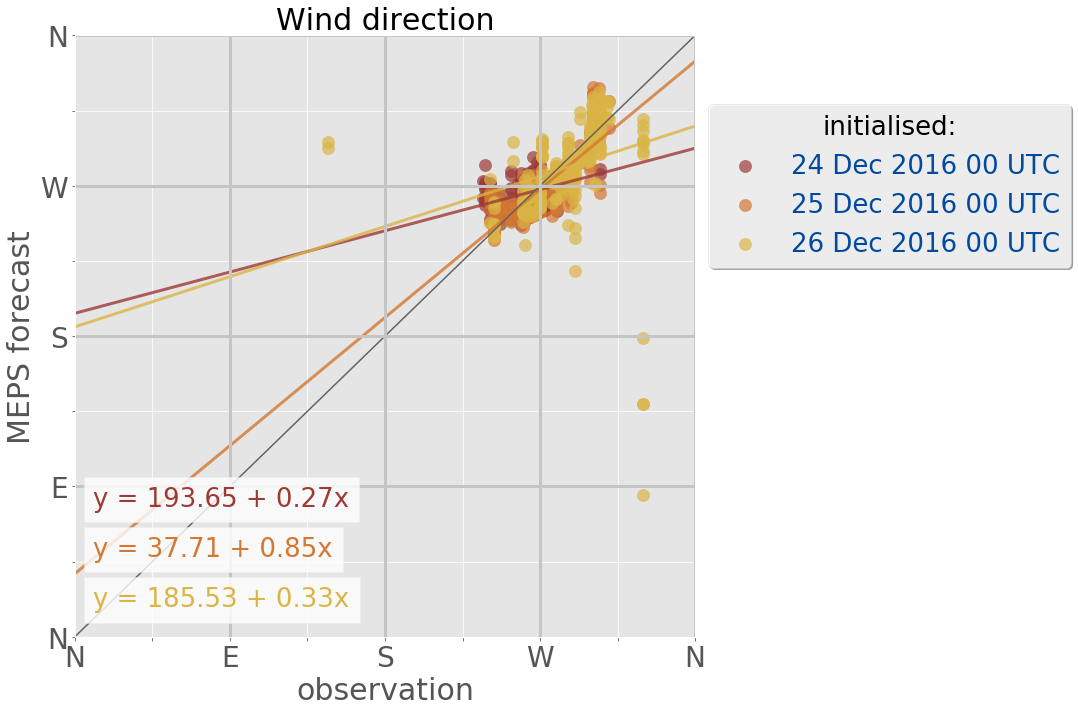
\includegraphics[
		width=\textwidth]{./fig_sfc_wd/obs_model_20161224_26_00}
		\caption{}\label{fig:scat:wd2426}
	\end{subfigure}
	
	% label
	\begin{subfigure}[b]{0.49\textwidth}
		\centering
		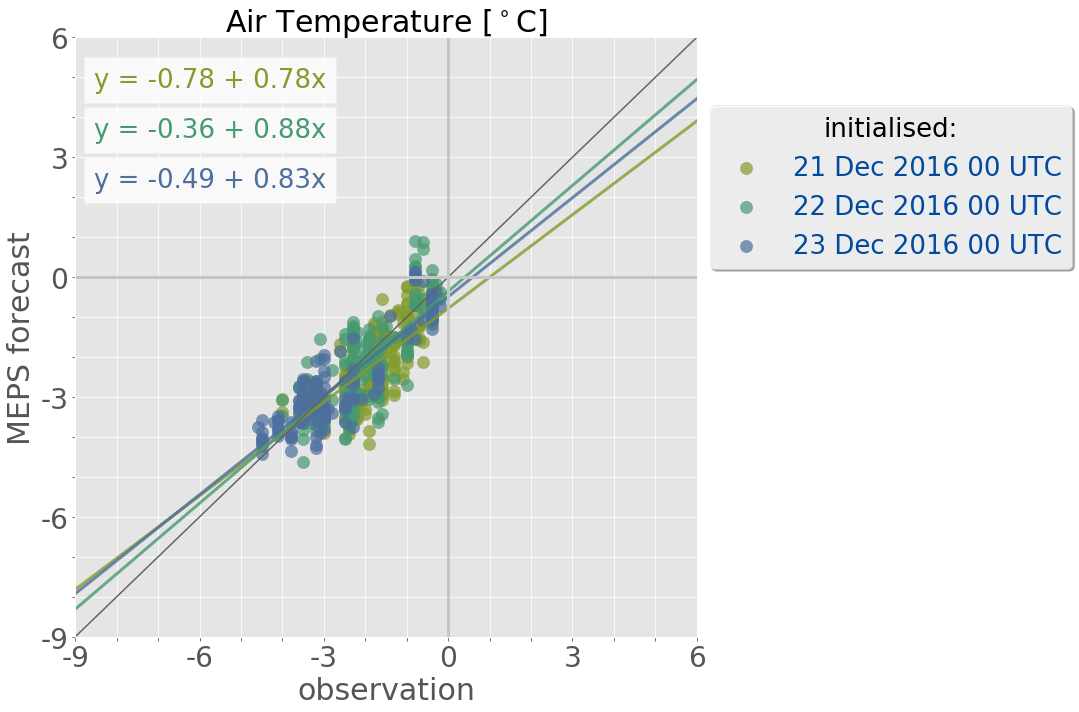
\includegraphics[trim={25.cm 15.5cm 0cm 3.6cm},clip,
		width=0.8\textwidth]{./fig_sfc_temp/obs_model_20161221_23_00_label}
	\end{subfigure}
	\begin{subfigure}[b]{0.49\textwidth}
		\centering
		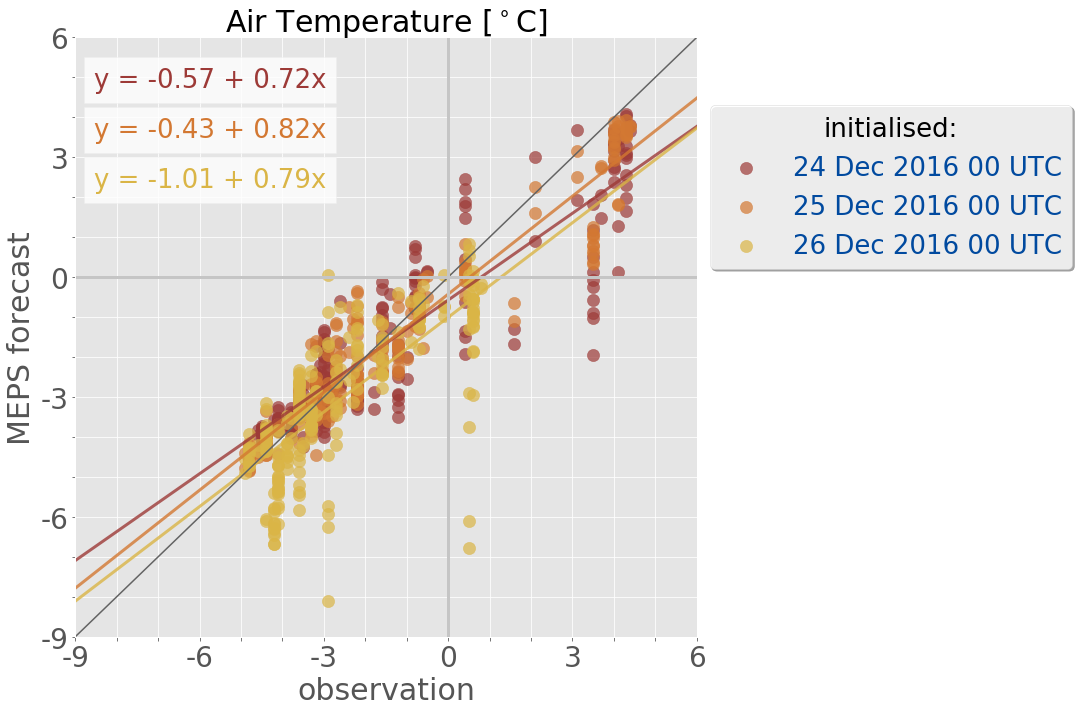
\includegraphics[trim={25.cm 15.5cm 0cm 3.6cm},clip,
		width=0.8\textwidth]{./fig_sfc_temp/obs_model_20161224_26_00_label}
	\end{subfigure}
	\caption{\textit{(As \Cref{fig:scat:SLP}.)} From top to bottom: (\protect\subref{fig:scat:temp2123}, \protect\subref{fig:scat:temp2426}) \SI{2}{\metre} air temperature, (\protect\subref{fig:scat:wd2123}, \protect\subref{fig:scat:wd2426}) \SI{10}{\metre} wind direction.} \label{fig:scat:T_WD}
\end{figure}
\begin{figure}%\ContinuedFloat
	% sfc ws
	\begin{subfigure}[b]{0.49\textwidth}
		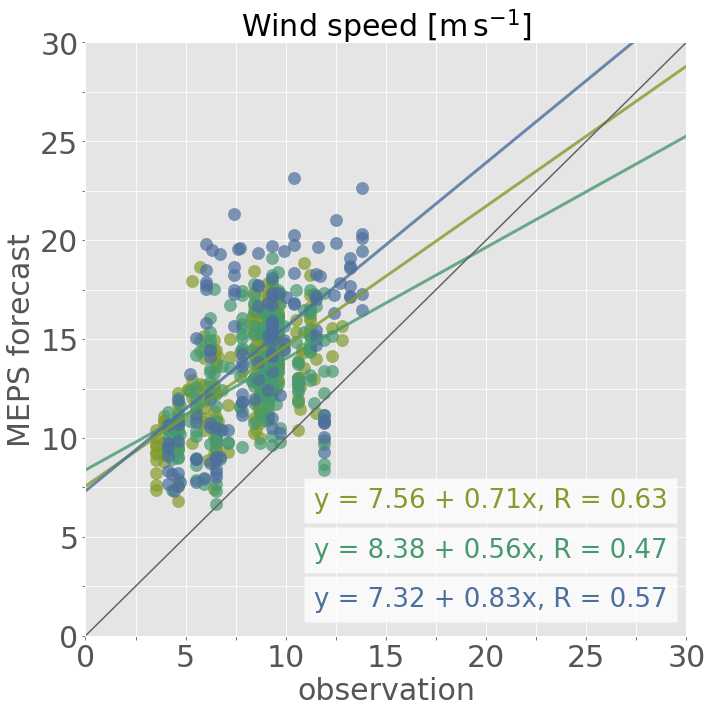
\includegraphics[
		width=\textwidth]{./fig_sfc_ws/obs_model_20161221_23_00}
		\caption{}\label{fig:scat:ws2123}
	\end{subfigure}
	%
	\begin{subfigure}[b]{0.49\textwidth}
		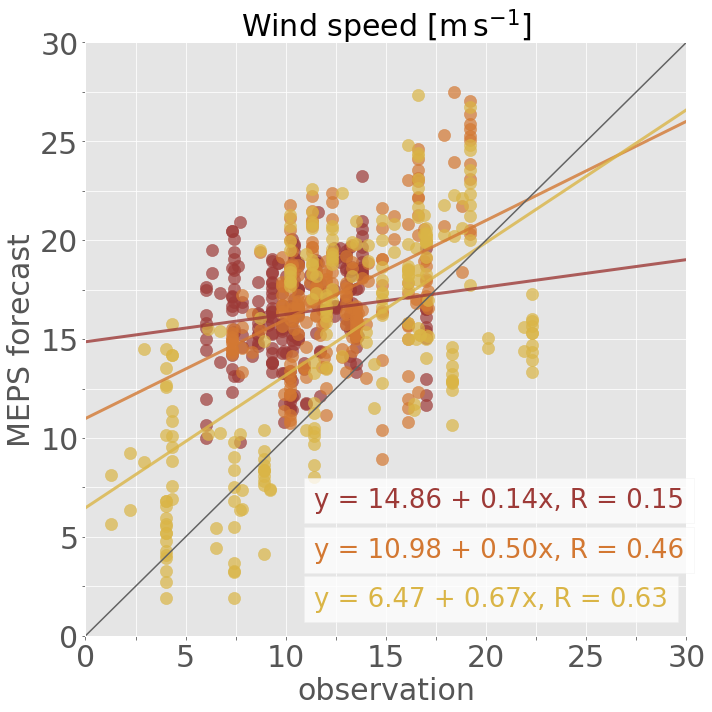
\includegraphics[
		width=\textwidth]{./fig_sfc_ws/obs_model_20161224_26_00}
		\caption{}\label{fig:scat:ws2426}
	\end{subfigure}
	% sfc precip
	\begin{subfigure}[b]{0.49\textwidth}
		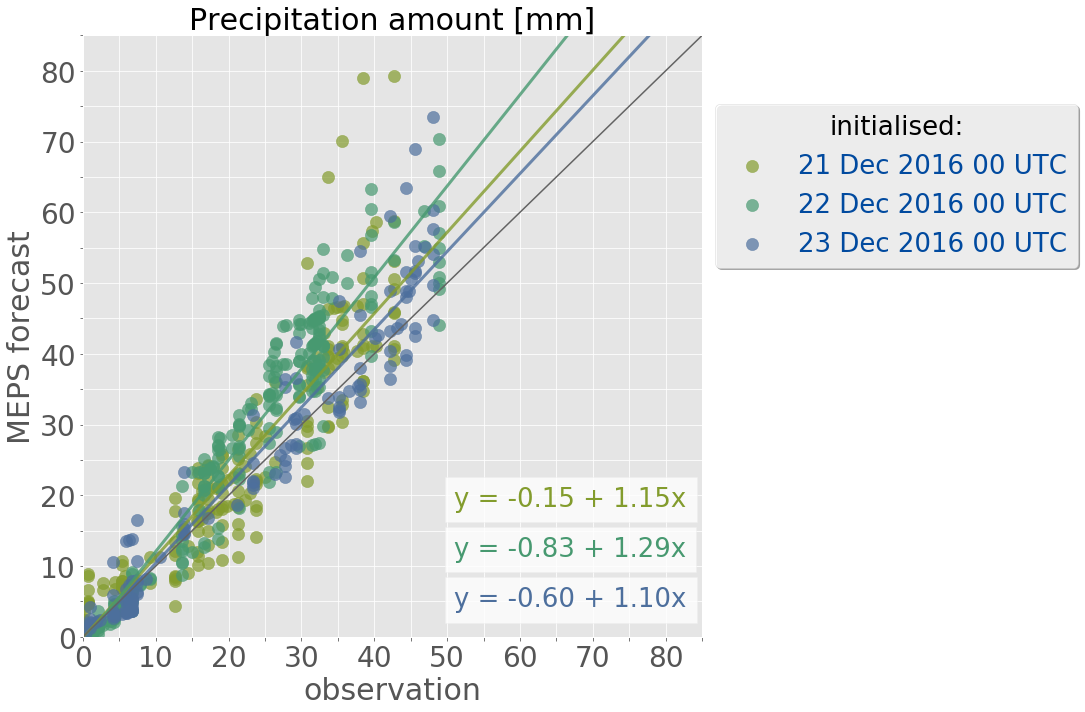
\includegraphics[
		width=\textwidth]{./fig_sfc_precip/obs_model_20161221_23_00}
		\caption{}\label{fig:scat:precip2123}
	\end{subfigure}
	%
	\begin{subfigure}[b]{0.49\textwidth}
		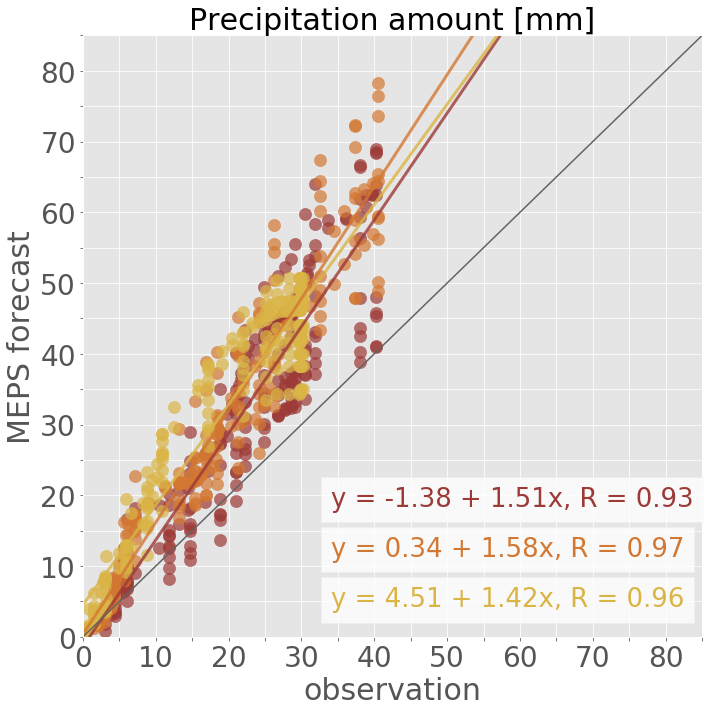
\includegraphics[
		width=\textwidth]{./fig_sfc_precip/obs_model_20161224_26_00}
		\caption{}\label{fig:scat:precip2426}
	\end{subfigure}
	% label
	\begin{subfigure}[b]{0.49\textwidth}
		\centering
		\includegraphics[trim={25.cm 15.5cm 0cm 3.6cm},clip,
		width=0.8\textwidth]{./fig_sfc_temp/obs_model_20161221_23_00_label}
	\end{subfigure}
	\begin{subfigure}[b]{0.49\textwidth}
		\centering
		\includegraphics[trim={25.cm 15.5cm 0cm 3.6cm},clip,
		width=0.8\textwidth]{./fig_sfc_temp/obs_model_20161224_26_00_label}
	\end{subfigure}
    \caption{\textit{(As \Cref{fig:scat:SLP}.)} From top to bottom: (\protect\subref{fig:scat:ws2123}, \protect\subref{fig:scat:ws2426}) \SI{10}{\metre} wind speed, (\protect\subref{fig:scat:precip2123}, \protect\subref{fig:scat:precip2426}) surface precipitation amount comparing double fence observations to \SI{48}{\hour} MEPS forecasts.} \label{fig:scat:WS_precip}
\end{figure}
%%%%%%%%%%%%%%%%%%%%%%%%%%%%%%%%%%%%%%%%%%%%%%
\noindent
\\
\\
Similar patterns as on \SI{23}{\dec} is seen for the evolution of the occluded front on \SI{26}{\dec} in the ECMWF analysis \Cref{fig:DT26} and \ref{fig:GP26}. In this case the low-pressure system was located north of Møre and Romsdal in the Norwegian Sea. In the morning the cyclone is located east of Iceland and in the course of the day it moves closer to the coast of Norway (\Cref{fig:DT26_18} and \ref{fig:GP26_18}). Before landfall at \SI{16}{\UTC}, a pressure decrease occurs at Haukeliseter (\Cref{fig:res:sfc_pres26}). During the development of the occluded front, the pressure reaches its lowest point of \SI{985}{\hPa} (\Cref{fig:res:sfc_pres26}) and increases afterwards during the dissipation of the 2016 Christmas storm. 
%% Pressure, temperature, and wind changes for the occlusion transition were already forecasted for initialisations on \SI{25}{\dec} (\Cref{fig:res:sfc_pres25}, \subref{fig:res:sfc_temp25}, \subref{fig:res:sfc_wd25}, \subref{fig:res:sfc_ws25}), only wind speed and precipitation seem not to agree with the observations at Haukeliseter. 
\\
Since the cyclone was surrounded by colder air (south of the low-pressure system in \Cref{fig:DT26}), first a drop and then an increase of temperature were observed and forecasted by MEPS (\Cref{fig:res:sfc_temp26}). An indication of the occlusion evolution is also visible in the \SI{10}{\metre} wind observations and MEPS predictions in \Cref{fig:res:sfc_wd26} and \subref{fig:res:sfc_ws26}. 
On \SI{26}{\dec} at \SI{0}{\UTC}, the low pressure system is east of Iceland (not shown), moving closer into the Norwegian Sea by \SI{12}{\UTC} (\Cref{fig:DT26} and \ref{fig:GP26}). 
Surface westerly winds are associated to the cyclone in the Norwegian Sea, and impinging on the West coast of Norway \Cref{fig:GP26}. The \SI{10}{\metre} wind measurement and MEPS forecast in \Cref{fig:res:sfc_wd26} and \ref{fig:res:sfc_ws26}, show a westerly gale of up to \SI{18}{\mPs} at Haukeliseter before \SI{12}{\UTC}.
The centre of the occluded front is located over Norway at \SI{18}{\UTC}, and the pronounced surface pressure gradient, in \Cref{fig:GP26_18}, indicate an increase in surface wind with a north-west wind direction. During this transition of the occlusion, the wind direction changes to north-west with higher observed wind speeds up to \SI{20}{\mPs} (\Cref{fig:res:sfc_wd26} and \ref{fig:res:sfc_ws26}). 
\\
Throughout the day light to moderate precipitation is continuing until the occlusion passage is seen in \Cref{fig:res:sfc_precip26}.
Heavy precipitation related to the occlusion, around \SI{16}{\UTC}, is followed by moderate to light precipitation on \SI{26}{\dec}. 
\\
%%%%%%% image liquid obs particle %%%%%%%%%%%%%%%%
\begin{figure}[t]
	\centering
	\includegraphics[%trim={45.cm 30.cm 13cm 35cm},clip,
	width=0.8\textwidth]{./MASC_obs/Masc_obs_liquid_2512}
	\caption{MASC images of falling water drops observed on \SI{25}{\dec} at \SI{17}{\UTC} from three different angles. Not all parts of the liquid sphere are equally illuminated.}\label{fig:res:obs_masc}
\end{figure}
%%%%%%%%%%%%%%%%%%%%%%%%%%%%%%%%%%%%%%%%%%%%%%
\\
On \SI{23}{\dec} a cyclone is south of Iceland (\Cref{fig:weather:23}) and precipitation was associated to the transition of the occlusion. 
While \SI{26}{\dec} precipitation was associated with the landfall of an occlusion. \SI{25}{\dec} was marked by the transition of a warm sector. The ECMWF analysis shows a pronounced upper level ridge at the dynamic tropopause (\Cref{fig:DT25}). The cyclone core is south east of Iceland in \Cref{fig:DT25} with two associated frontal boundaries. While the warm front is approaching the west coast, the cold front is north-west of Great Britain. In \Cref{fig:GP25}, the tail of the cold front moved into lower latitudes, following the slowdown of the front, leading to a stationary frontal boundary. Furthermore, the mid-latitude jet is aligned with the surface frontal boundaries (\Cref{fig:DT25}), while the Haukeliseter site is located below the the midlatitudal jet (\Cref{fig:GP25}). %This leads to rising motion at the surface.
\\
Neither pressure nor wind observations and forecasts in \Cref{fig:res:sfc_pres25}, \subref{fig:res:sfc_wd25}, and \subref{fig:res:sfc_ws25}, indicate the evolution of any frontal boundary. The only indication of a transition could be seen in the increase and decrease of temperature afterwards at \SI{11}{\UTC} until \SI{21}{\UTC} (\Cref{fig:res:sfc_temp25}). In \Cref{fig:res:sfc_wd25}, a small wind direction change from west to north-west is observed by the wind mast at \SI{10}{\UTC}. This is not forecasted by MEPS, as it rather estimated strong westerly winds.
\\
Particle images taken by the MASC are available on \SI{25}{\dec}, during the transition of the warm sector in \Cref{fig:res:obs_masc}. Without theses images taken around \SI{17}{\UTC} it would only be possible to verify that liquid precipitation occurred with the optical precipiation detectors at the Haukeliseter site. Together with the increase in surface temperature (\Cref{fig:res:sfc_temp25}) it can be concluded that the warm sector of the Christmas 2016 event passed by the measurement site.
%\textcolor{red}{KICKI: Should I include the DIANA analysis maps? But the meteorologist also use ECMWF to make them!}
%
\\
\\
The comparison between the ECMWF analysis (\Cref{sec:largeScale}) and the observations at the measurement site (\Cref{fig:res:sfc_obs_meps}), allow to conclude that the ensemble member forecast system MEPS covers the prediction of large scale weather systems like occlusions and fronts, as well as liquid precipitation at the surface. 
\\
The scatter plots for observations and MEPS forecasts show good correlation for most variables (\Cref{fig:scat:SLP,fig:scat:T_WD,fig:scat:WS_precip}).
The best agreement for pressure is reached on \SI{26}{\dec} (\Cref{fig:res:sfc_pres26}), when the Christmas storm hit land and dissipated after the evolution of the occlusion at \SI{16}{\UTC}. \citet{dahlgren_comparison_2013} showed an improvement of sea level pressure forecast for AROME, by including large scale boundary conditions for ECMWF into the regional model. The observation-model comparison by \citet{dahlgren_comparison_2013} showed a decrease of pressure bias with lead time after \SI{24}{\hour} with the use of pressure mixing. 
Since surface pressure is in good agreement with the observations, it is assumed that the warm front did not pass through Haukeliseter on \SI{25}{\dec} and only the warm sector associated with the 2016 Christmas storm is observed. This shows a quite detailed forecast ability of MEPS, as from the ECMWF analysis, in \Cref{fig:DT25}, it is not quite clear if the warm front could have passed through. To be sure that the warm front did not pass through Haukeliseter, or whether it is a predictive error of MEPS, surface pressure, temperature and wind should be compared to the nearest grid point of the global forecast model ECMWF to verify this result.
\\
\Cref{fig:scat:temp2426} displays a moderate correlation between observation and the \SI{48}{\hour} MEPS ensemble member forecast system. In general, MEPS underestimates the observed \SI{2}{\metre} air temperature, but MEPS estimated the temperature changes at the correct occurrence for \num{23}, \num{25}, and \SI{26}{\dec}. 
\\
This thesis uses only one extreme event during Christmas 2016 at Haukeliseter. 
\Cref{fig:bias:temp} shows warm and cold biases for \num{23} and \SI{26}{\dec}, respectively for Haukeliseter during the Christmas 2016 storm. On \SI{25}{\dec}, within the warm sector, a cold bias was observed, underestimating the temperature when compared to the observation. The forecasts for \num{23}, \num{25}, and \SI{26}{\dec} show calculated mean absolute error values (\Cref{eq:MAE}) below \SIlist{1}{\kelvin} in \Cref{fig:MAE:temp}. 
In the verification report of Met-Norway MEPS deterministic forecast is verified against observations for December 2016 to February 2017 \citep{homleid_verification_2016}. For December 2016 the \SI{2}{\metre} air temperature had no bias within the Norwegian model domain. The Norwegian mean absolute error for \SI{2}{\metre} air temperature was \SI{1.6}{\kelvin} \citep{homleid_verification_2016}. The mean absolute error for the Christmas 2016 storm is within the Norwegian December mean for the deterministic forecast. This does not necessarily show how well the forecast predicted the extreme event, since only one storm is studied at one site in Norway.
The previous operational deterministic forecast model AROME-MetCoOp showed a cold bias of \SI{2}{\metre} temperature for the Norwegian mean, during winter 2013 with the introduction of AROME-Norway and later AROME-MetCoOp \citep{muller_arome-metcoop:_2017}. 
The mean error for the Norwegian model domain of AROME-MetCoOP estimated by \citet{muller_arome-metcoop:_2017} is smaller than \SI{1.8}{\kelvin} for the surface \SI{2}{\metre} air temperature in December 2014. 
%The new ensemble forecast system MEPS shows a reduction of mean errors for the Christmas 2016 extreme event, when compared to the Norwegian mean of AROME-MetCoOp.
\\
%%% image bias %%%%%%%%%%%%%%%%%%%%%%%%%%%%%%%%%%%%%
\begin{figure}[H]%\ContinuedFloat
	\centering
	% pres
	\begin{subfigure}[b]{\textwidth}
		\includegraphics[trim={0cm 0cm 0cm 9.5cm},clip,width=\textwidth]{./fig_sfc_pressure/ME_20161220_26_00}
		\caption{}\label{fig:bias:pres}
	\end{subfigure}
	% temp
	\begin{subfigure}[b]{\textwidth}
		\includegraphics[trim={0cm 0cm 0cm 9.5cm},clip,width=\textwidth]{./fig_sfc_temp/ME_20161220_26_00}
		\caption{}\label{fig:bias:temp}
	\end{subfigure}
	% wd
	\begin{subfigure}[b]{\textwidth}
		\includegraphics[trim={0cm 0cm 0cm 9.5cm},clip,width=\textwidth]{./fig_sfc_wd/ME_20161220_26_00}
		\caption{}\label{fig:bias:wd}
	\end{subfigure}
	% \end{figure}
	% \begin{figure}[ht!]\ContinuedFloat
	\centering
	% ws
	\begin{subfigure}[b]{\textwidth}
		\includegraphics[trim={0cm 0cm 0cm 9.5cm},clip,width=\textwidth]{./fig_sfc_ws/ME_20161220_26_00}
		\caption{}\label{fig:bias:ws}
	\end{subfigure}
	% \end{figure}
	% \begin{figure}\ContinuedFloat
	% \centering
	%         % precip
	% 		\begin{subfigure}[b]{0.75\textwidth}
	% 			\includegraphics[width=\textwidth]{./fig_sfc_precip/ME_20161220_26_00}
	% 			\caption{}\label{fig:bias:precip}
	% 		\end{subfigure}
	% precip 12h
	\begin{subfigure}[b]{\textwidth}
		\includegraphics[trim={0cm 0cm 0cm 9.5cm},clip,width=\textwidth]{./fig_sfc_precip/ME_20161220_26_00}
		\caption{}\label{fig:bias:precip12}
	\end{subfigure}
	\caption{{Mean error of surface variables for all ten ensemble members at Haukeliseter, initialisations at \SI{0}{\UTC} with lead times from \SIrange{6}{24}{\hour}. From top to bottom, sea level pressure (\protect\subref{fig:bias:pres}), \SI{2}{\metre} air temperature (\protect\subref{fig:bias:temp}), \SI{10}{\metre} wind direction (\protect\subref{fig:bias:wd})},  \SI{10}{\metre} wind speed (\protect\subref{fig:bias:ws}), precipitation accumulation for 
		%\SI{48}{\hour} (\protect\subref{fig:bias:precip}) and 
		\SI{12}{\hour} surface accumulation (\protect\subref{fig:bias:precip12}). } \label{fig:bias}
\end{figure}
%%%%%%%%%%%%%%%%%%%%%%%%%%%%%%%%%%%%%%%%%%%%%%%%%%%%%%%%%%%%%
\noindent
\\
During the Christmas storm 2016 high wind speeds were observed at the Haukeliseter site (\Cref{fig:res:sfc_ws23}, \ref{fig:res:sfc_ws25}  and \ref{fig:res:sfc_ws26}).
According to \citet{muller_arome-metcoop:_2017} high wind speeds are significantly better simulated for AROME-MetCoOp compared to ECMWF's forecast for the model domain. MEPS predictions of wind speed in \Cref{fig:res:sfc_ws23}, \ref{fig:res:sfc_ws25}, and \ref{fig:res:sfc_ws26} still display an overestimation of wind speeds throughout the event. Furthermore, the correlation of observations and wind speed in \Cref{fig:scat:ws2123} and \subref{fig:scat:ws2426} show an overestimation for stronger wind speeds on \num{24} to \SI{26}{\dec} than for \num{21} to \SI{23}{\dec}. 
The mean error for wind speed during the Christmas storm is ranging from \SIrange{0}{7}{\mPs} for \SI{48}{\hour} lead time (\Cref{fig:bias:ws}).
During the extreme storm, the highest mean absolute error of \SI{10}{\mPs} occurs for initialisations on \SI{24}{\dec} (\Cref{fig:MAE:ws}).
\\
The inaccuracy for wind speeds is an already known difficulty in the deterministic version of MEPS \citep{muller_arome-metcoop:_2017}. \citet{muller_arome-metcoop:_2017} presented, that AROME-MetCoOp wind speed prediction generally agreed better with observations for wind speeds between \SIrange{3}{13}{\mPs} than ECMWF forecasts did, showing the advantage of a high-resolution weather model. Furthermore, with increasing wind speed the forecast accuracy for the Norwegian mean decreased with a mean absolute error below \SI{2}{\mPs} for \SIrange{6}{24}{\hour} lead times, in December 2014 in AROME-MetCoOp. \citet{muller_arome-metcoop:_2017} case study showed a slight underestimation of ECMWF \SI{10}{\metre} wind compared to the Norwegian AROME-MetCoOp forecast for February 2015. %, but still overestimates MEPS the wind.
On \SI{24}{\dec}, the mean absolute error is more than fives times as high as the monthly averaged value for the Norwegian forecast domain (\SI{2}{\mPs} for \SIrange{6}{24}{\hour} forecast time) from \citet{muller_arome-metcoop:_2017}. 
In December 2016, the mean absolute error for the Norwegian mean of the deterministic forecast was \SI{2}{\mPs} \citep{homleid_verification_2016}.
The difference between the mean absolute error during the event and the monthly averages of Met-Norway, is firstly related to the comparison of a long term study of \citet{muller_arome-metcoop:_2017}. Secondly to a month average mean absolute for the Norwegian model domain \citep{muller_arome-metcoop:_2017,homleid_verification_2016}, and third to the location of Haukeliester (orographic effect, \Cref{sec:res:oro_infl}). 
\\
Haukeliseter is a measurement site exposed to high wind speeds \citep{wolff_measurements_2013,wolff_derivation_2015}. The ensemble prediction system MEPS seems to still have issues forecasting the wind speed correctly in mountainous terrain.
A detailed insight to the orographical wind influence will be discussed in \Cref{sec:res:oro_infl}. 
\\
Pressure, temperature, and wind changes for the occlusion transition on \SI{26}{\dec} were already forecasted for initialisations on \SI{25}{\dec} (\Cref{fig:obs_meps:25}), only wind speed and precipitation seem not to agree with the observations at Haukeliseter. The same is true for \SI{25}{\dec}, when the warm sector passes through Haukeliseter. 
\\
\Cref{fig:obs_meps:21,fig:obs_meps:22,fig:obs_meps:23,fig:obs_meps:24,fig:obs_meps:25,fig:obs_meps:26}\subref{fig:res:sfc_precip23} illustrate the surface precipitation amount observed and predicted by MEPS for Haukeliseter. MEPS overestimation is shown for precipitation when the cyclone intensifies and gets closer to Norway on \num{24}, \num{25} and \SI{26}{\dec}. The surface observations and MEPS predictions in \Cref{fig:scat:precip2123} and \subref{fig:scat:precip2426} show an overestimate for \num{24}, \num{25} and \SI{26}{\dec}, whereas on \num{21}, \num{22}, and \SI{23}{\dec} the surface accumulation is balanced for  predictions up to \SI{30}{\mm}. Any reasons for the overestimation of precipitation accumulation on the ground will be further analysed and discussed in \Cref{sec:sfc_acc}. 
% \textcolor{red}{I HAVE TO SOMEHOW MERGE THIS IN, BUT HOW? What could be still a weakness that the model overestimates the wind speed? In \citet{muller_arome-metcoop:_2017}: change from ECOCLIMAP1 because the surface roughness was too low and followed high wind speeds? Is this still the case for MEPS? High wind speeds followed also from wrongly adressed 'permanent snow'. Do not use 'orographi drag' in AROME-MetCoOp, could that lead to the too high estimated wind? When 'canopy drag' was changed saw increase in SBL drag which followed a decrease in wind speed. But AROME-MetCoOp is able to forecast high wind speeds, while ECMWF is not.}
%%%%%%%%%%%%%%%%%%%%%%%%%%%%%%%%%%%%%%%%%%%%%%%%%%%%%%%%%%%%%%
\begin{figure}[H]%\ContinuedFloat
	\centering
	% pres
	\begin{subfigure}[b]{\textwidth}
		\includegraphics[trim={0cm 0cm 0cm 9.5cm},clip,width=\textwidth]{./fig_sfc_pressure/MAE_20161220_26_00}
		\caption{}\label{fig:MAE:pres}
	\end{subfigure}
	% temp
	\begin{subfigure}[b]{\textwidth}
		\includegraphics[trim={0cm 0cm 0cm 9.5cm},clip,width=\textwidth]{./fig_sfc_temp/MAE_20161220_26_00}
		\caption{}\label{fig:MAE:temp}
	\end{subfigure}
	% wd
	\begin{subfigure}[b]{\textwidth}
		\includegraphics[trim={0cm 0cm 0cm 9.5cm},clip,width=\textwidth]{./fig_sfc_wd/MAE_20161220_26_00}
		\caption{}\label{fig:MAE:wd}
	\end{subfigure}
	% \end{figure}
	% \begin{figure}\ContinuedFloat
	\centering
	% ws
	\begin{subfigure}[b]{\textwidth}
		\includegraphics[trim={0cm 0cm 0cm 9.5cm},clip,width=\textwidth]{./fig_sfc_ws/MAE_20161220_26_00}
		\caption{}\label{fig:MAE:ws}
	\end{subfigure}
	% \end{figure}
	% \begin{figure}\ContinuedFloat
	% \centering
	%         % precip
	%         \begin{subfigure}[b]{0.75\textwidth}
	% 			\includegraphics[width=\textwidth]{./fig_sfc_precip/MAE_20161220_26_00}
	% 			\caption{}\label{fig:MAE:precip}
	% 		\end{subfigure}
	% precip 12h
	\begin{subfigure}[b]{\textwidth}
		\includegraphics[trim={0cm 0cm 0cm 9.5cm},clip,width=\textwidth]{./fig_sfc_precip/MAE_20161220_26_00}
		\caption{}\label{fig:MAE:precip12}
	\end{subfigure}
	\caption{Mean absolute error (\protect\subref{fig:MAE:pres}, \protect\subref{fig:MAE:temp}, \protect\subref{fig:MAE:wd}, \protect\subref{fig:MAE:ws}, \protect\subref{fig:MAE:precip12}) of surface variables for all ten ensemble members at Haukeliseter, initialisations at \SI{0}{\UTC}, valid for \SI{48}{\hour}. From top to bottom, sea level pressure (\protect\subref{fig:MAE:pres}), \SI{2}{\metre} air temperature (\protect\subref{fig:MAE:temp}), \SI{10}{\metre} wind direction (\protect\subref{fig:MAE:wd}), \SI{10}{\metre} wind speed (\protect\subref{fig:MAE:ws}), precipitation accumulation for \SI{12}{\hour} surface accumulation (\protect\subref{fig:MAE:precip12}).}\label{fig:MAE}
\end{figure}
%%%%%%%%%%%%%%%%%%%%%%%%%%%%%%%%%%%%%%%%%%%%%%%%%%%%%%%%%%%%%%%%%%%%%%%%%%
\noindent
\\
\\
%\textcolor{red}{Write here about all days, a summary.}
Overall, for initialisations on \num{21} to \SI{23}{\dec} (\Cref{fig:scat:SLP,fig:scat:T_WD,fig:scat:WS_precip}) the forecast is best for all variables. 
The large-scale weather pattern seems to be more predictable as long as the weather situation is not extreme.
%on \SI{23}{\dec} than initialisations on \num{25} and \SI{26}{\dec}. 
The correlations for the forecasts between \num{24} and \SI{26}{\dec} (\Cref{fig:scat:SLP,fig:scat:T_WD,fig:scat:WS_precip}) suggest as MEPS may have difficulties predicting the intensification and associated pressure decrease of the Christmas 2016 storm at Haukeliseter. The prediction of pressure fits well on all days (\Cref{fig:scat:pres2123}, \subref{fig:scat:pres2426}) compared to temperature (\Cref{fig:scat:temp2123}, \subref{fig:scat:temp2426}), wind direction (\Cref{fig:scat:wd2123}, \subref{fig:scat:wd2426}), wind speed (\Cref{fig:scat:ws2123}, \subref{fig:scat:ws2426}), and precipitation (\Cref{fig:scat:precip2123}, \subref{fig:scat:precip2426}). The greatest difficulty MEPS has, is with the prediction of wind speed during the entire extreme event. The rainfall, however, fit well for \SI{23}{\dec} (\Cref{fig:res:sfc_precip23} and \ref{fig:scat:precip2123}), but MEPS has problems predicting the accumulation of surface precipitation amount correctly for the extreme days of the 2016 Christmas storm, \num{24} to \SI{26}{\dec} (\Cref{fig:res:sfc_precip25}, \ref{fig:res:sfc_precip26}, and \ref{fig:scat:precip2426}).
\\
\\
\Cref{fig:bias:pres}, \subref{fig:bias:temp} have shown good agreement of ensemble member forecasts with a small bias. It is not expected that ensemble members agree they should just give a variability around the observations, that is why ensemble member prediction exists. Based on the uncertainty in observations the solution space that is possible has to be understood (\Cref{sec:DIM:MEPS}). The model is not adjusted to present the extreme event particularly well as it is adjusted to span the full climatological range. For large weather situations which are considered as normal the observations have to be within the spread of the ensemble members \citep{owens_ecmwf_2018}. Because of the nature representing the climatology, ensemble members will either over- or under-estimate the risk of anomalous or extreme weather events.
\\
The extraction of an extreme weather event from an ensemble system is not always straightforward. For example, \SI{30}{\mm} precipitation during one day in December would not be extreme at the Norwegian West Coast, but would be at Haukeliseter during December.

%Nevertheless, extreme events should be within the spread of 
%For large weather situations which are considered as normal the observations have to be within the spread of the ensemble members. During extreme events, when large amount of precipitation is expected over short time the observation may not be within the ensemble spreads. 




